\section{Results}

\textbf{Note:} The visualizations presented here are preliminary versions that will be polished further before final submission. Some figures contain complementary plots that may not all be relevant to the main findings, and the current aesthetic quality will be improved.

This section presents the experimental validation of our multi-judge interpretability framework across three key dimensions: GAM model interpretability analysis, core performance comparison, and robustness evaluation under adversarial conditions.

\subsection{Main Results: Model Performance Comparison}

We compare our learned aggregation approaches against multiple baselines across 2,000 UltraFeedback samples, demonstrating significant improvements over naive aggregation methods.

\begin{figure}[htbp]
    \centering
    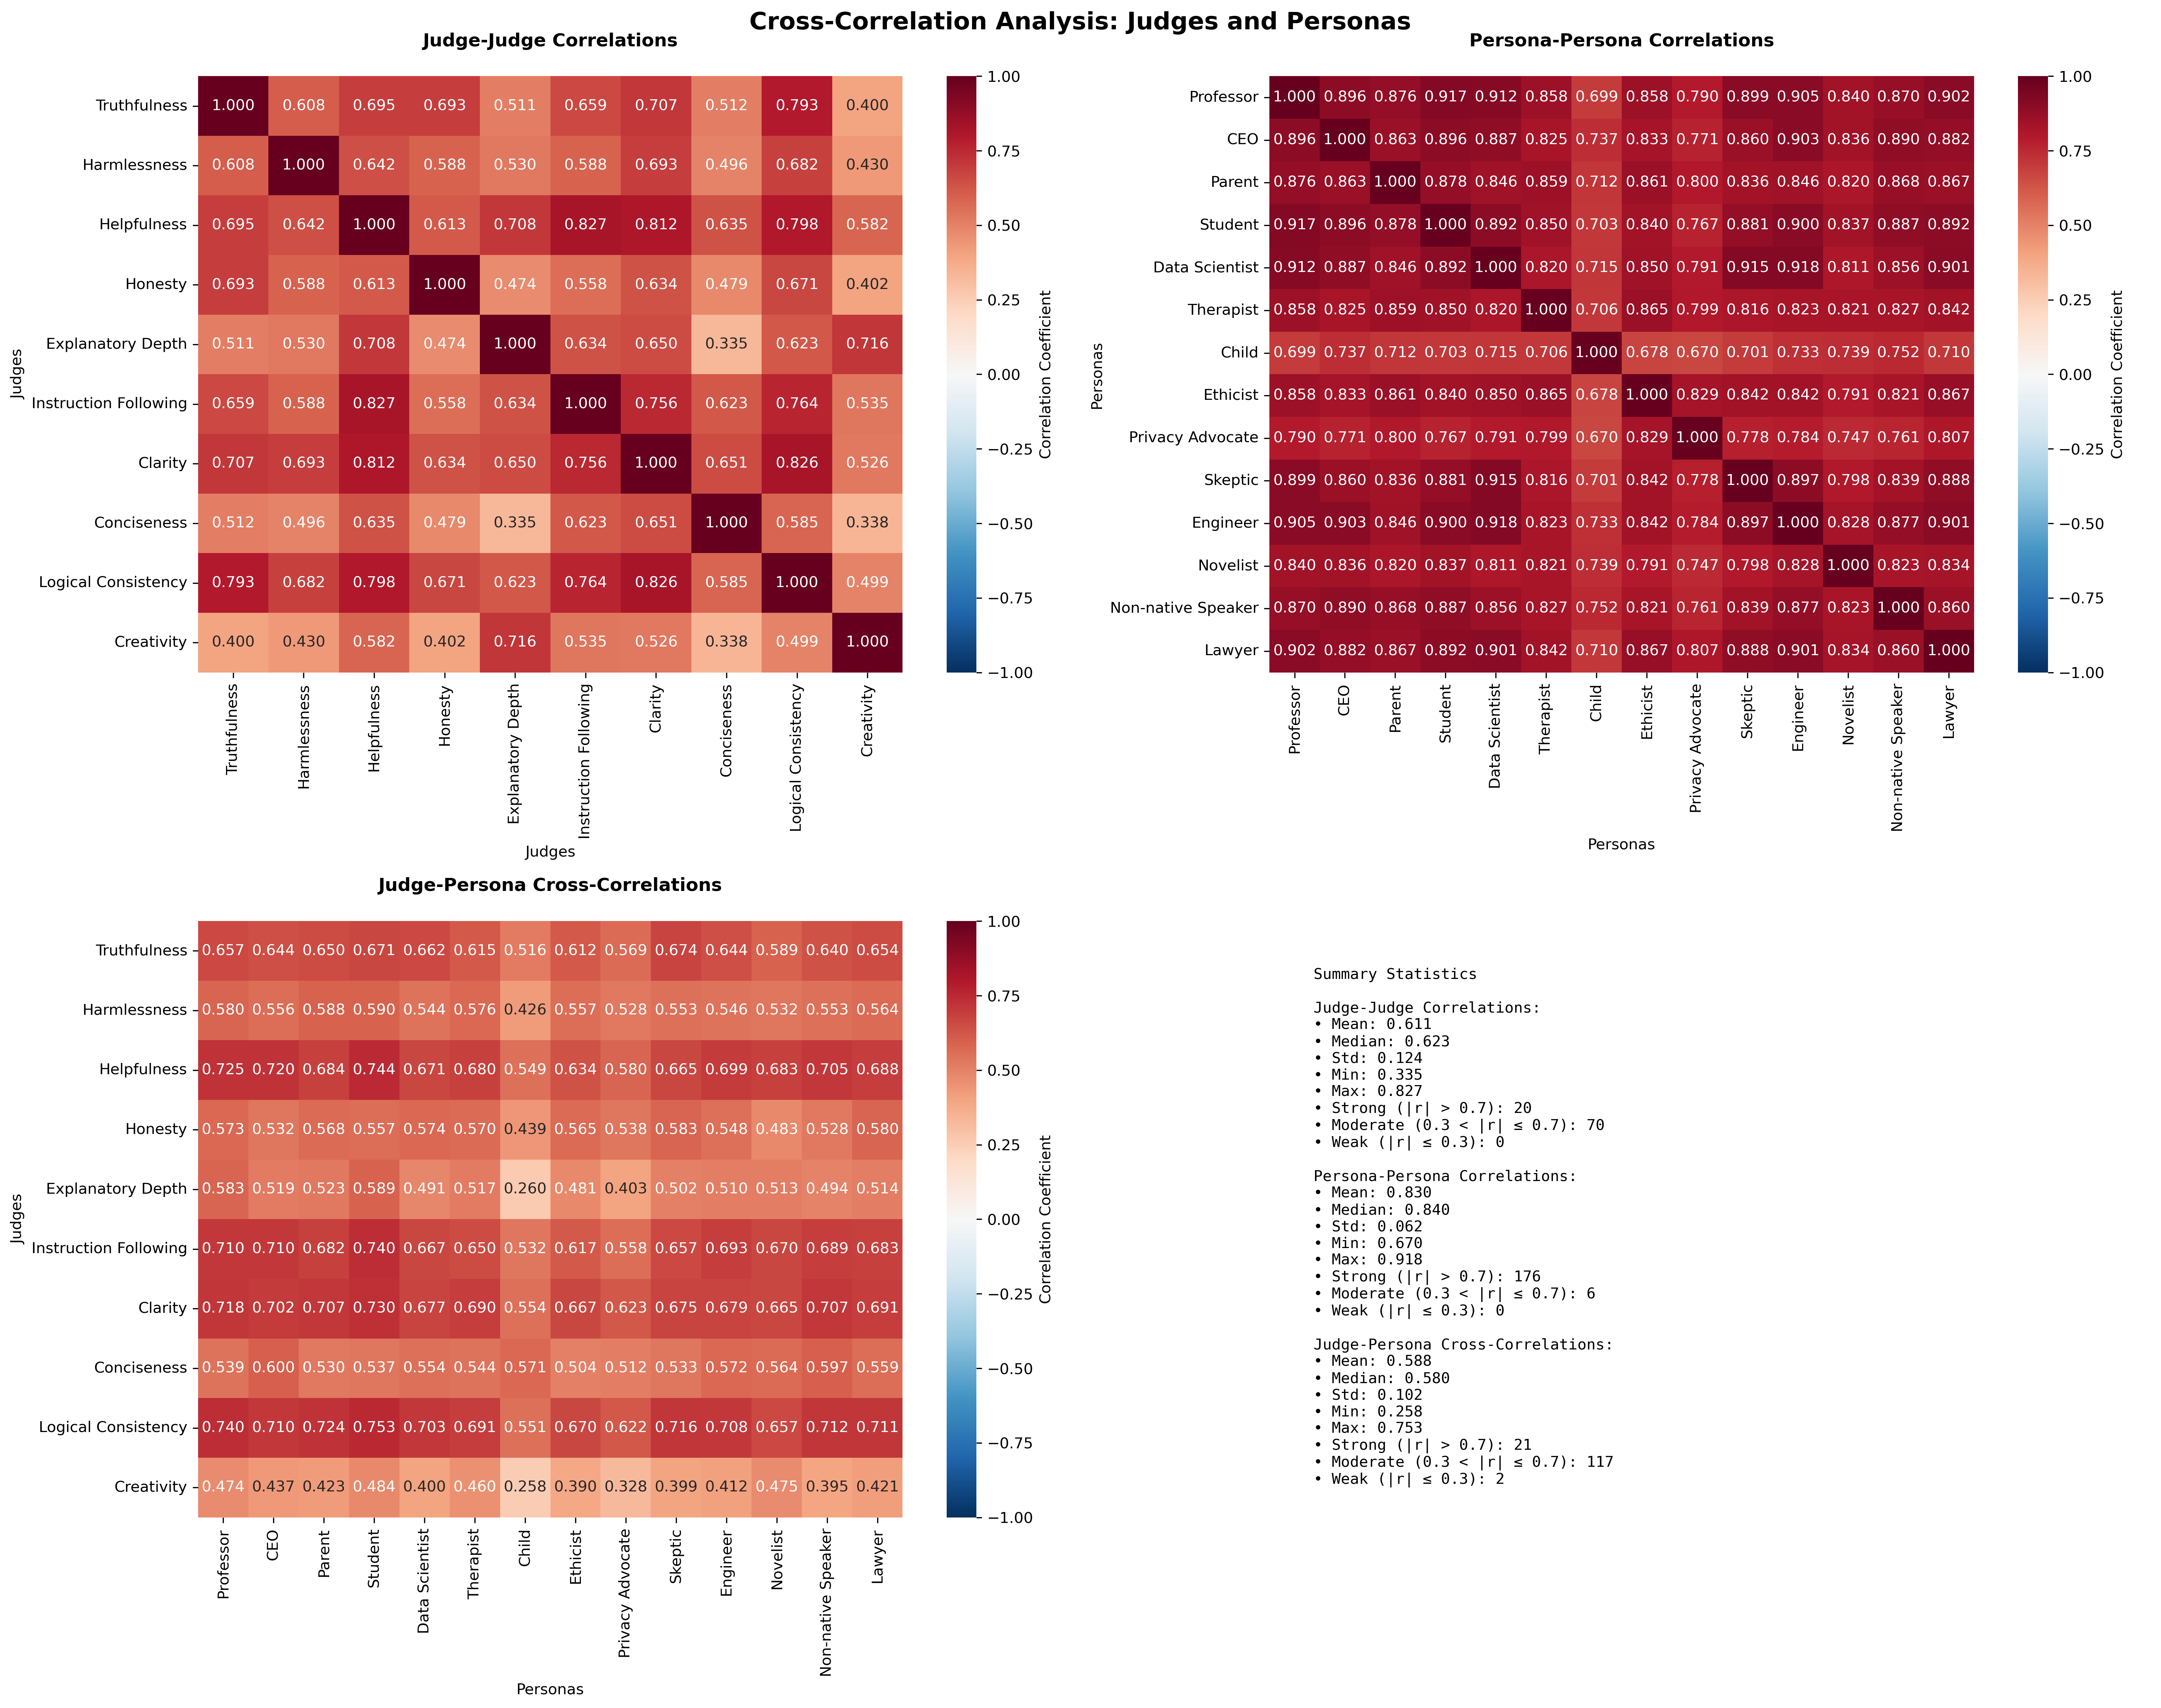
\includegraphics[width=0.8\textwidth]{Result Figures/Main Results/cross_correlation_heatmaps.png}
    \caption{Cross-Correlation Analysis: Judge agreement patterns revealing complementary evaluation dimensions. The analysis shows three correlation matrices: judge-judge correlations (top-left), persona-persona correlations (top-right), and judge-persona cross-correlations (bottom-left). Key findings from judge-judge correlations: (1) Truthfulness and Logical Consistency show strong correlation (0.73), (2) Helpfulness correlates well with Instruction Following (0.63) and Explanatory Depth (0.62), (3) Harmlessness operates relatively independently with lower correlations to other judges, and (4) Most correlations range from 0.2-0.7, indicating complementary but not redundant evaluation dimensions.}
    \label{fig:cross_correlation}
\end{figure}

\begin{figure}[htbp]
    \centering
    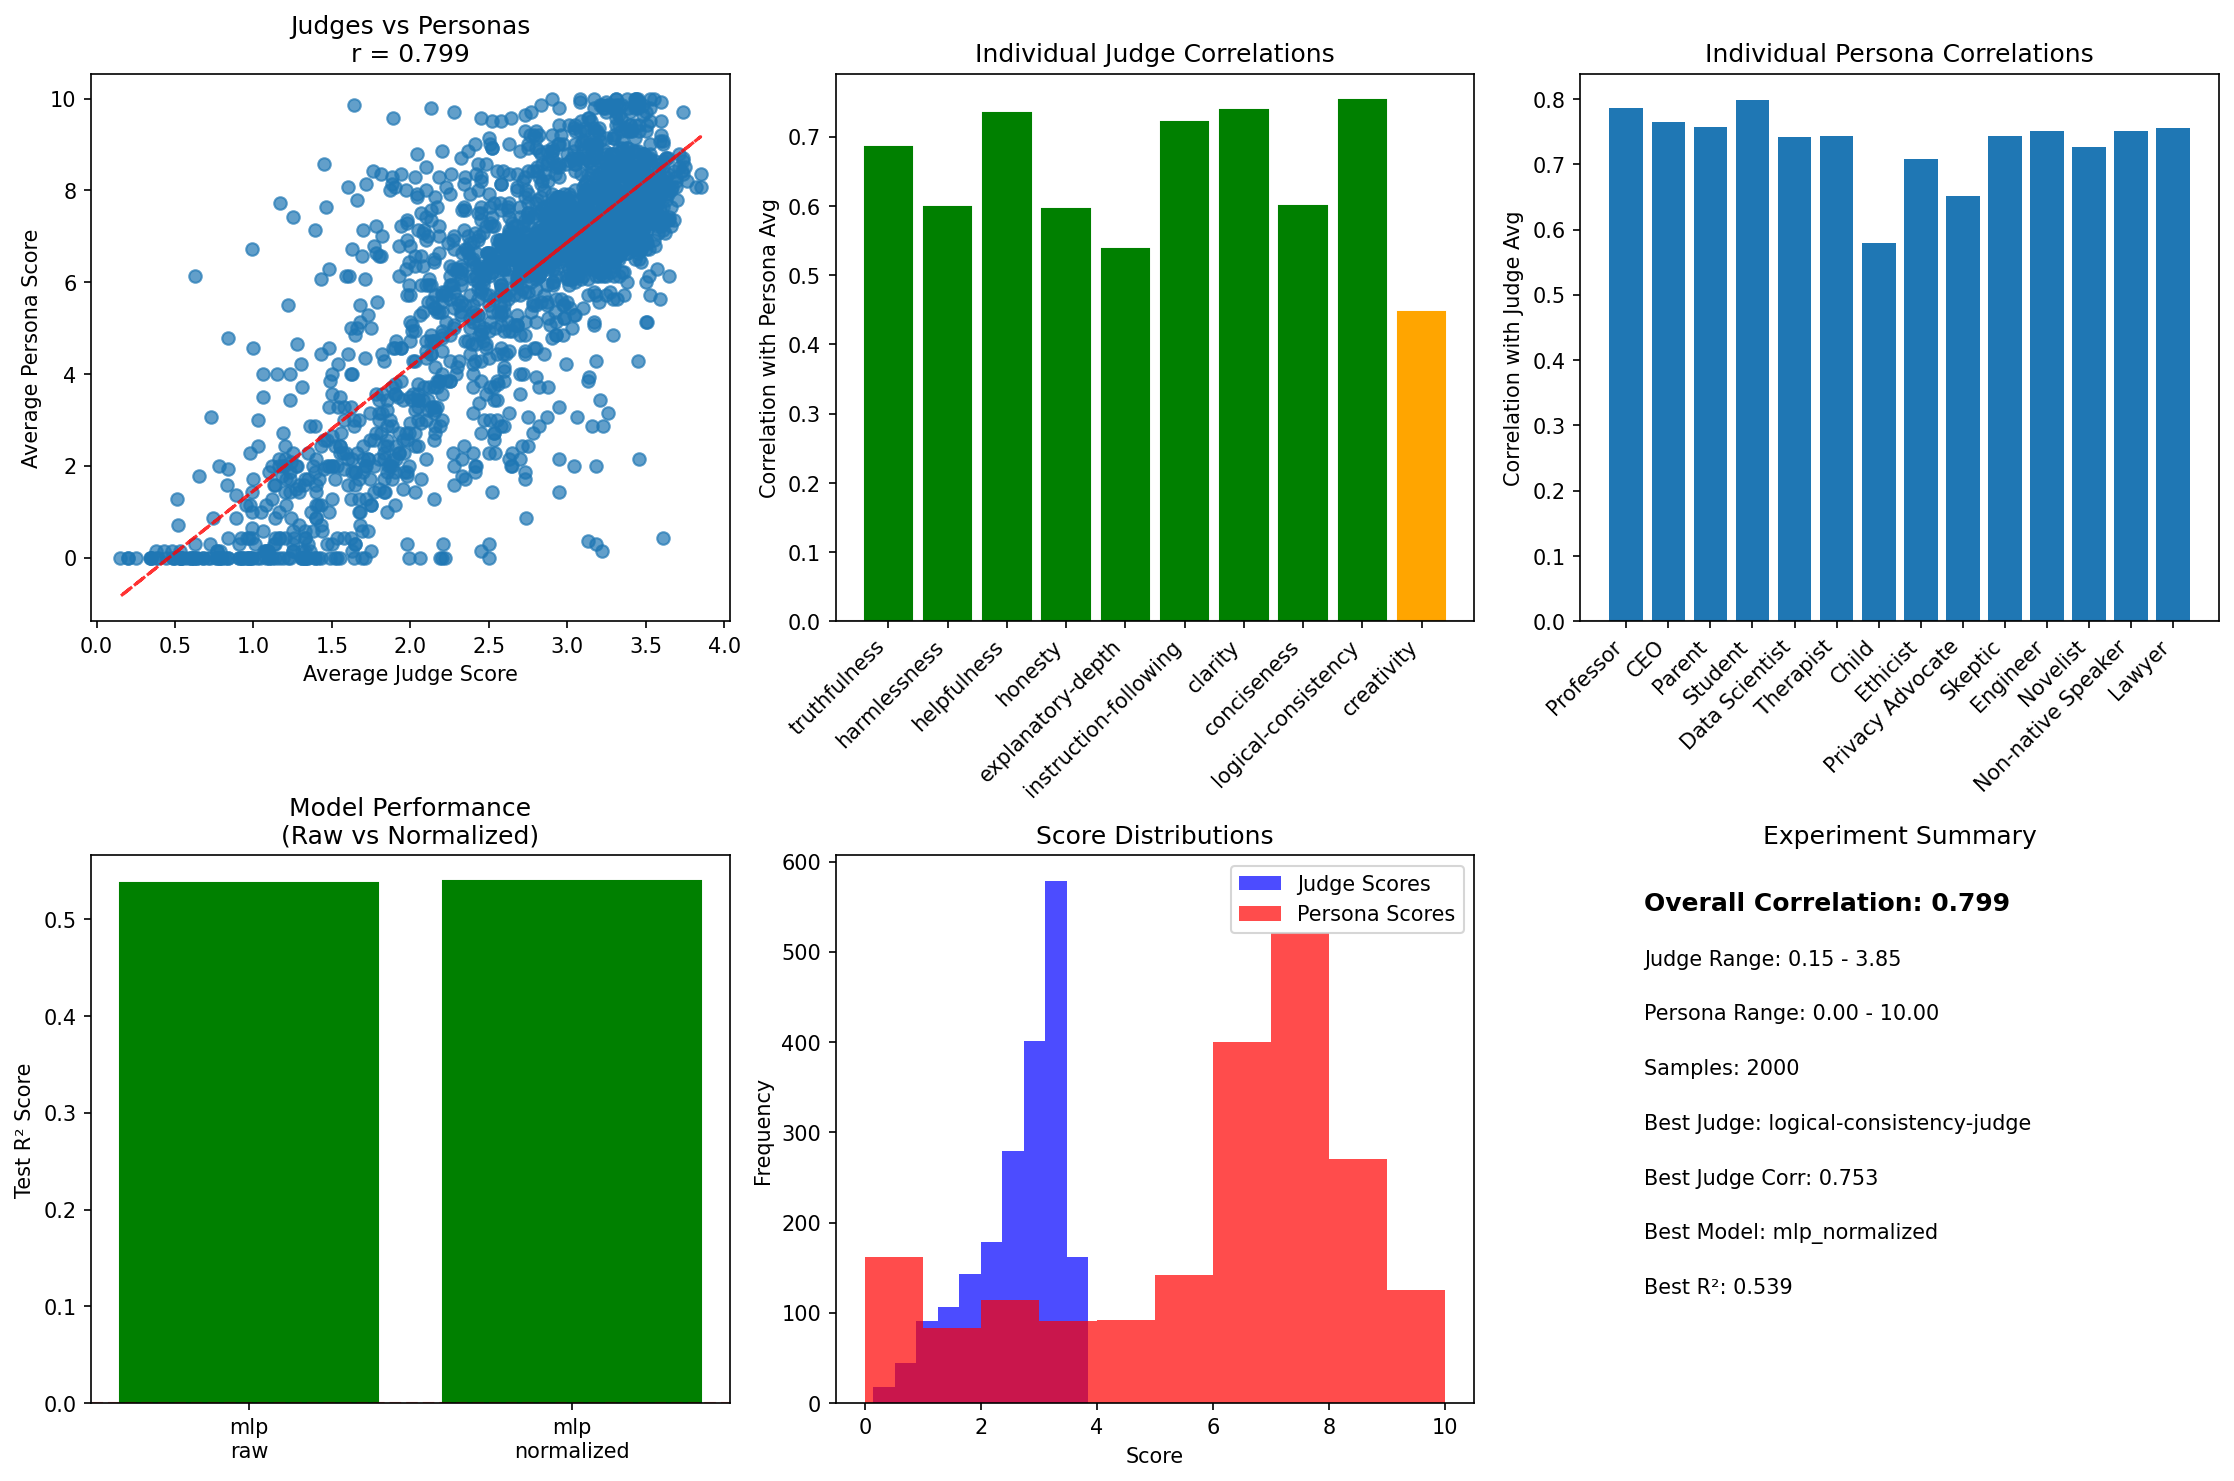
\includegraphics[width=0.8\textwidth]{Result Figures/Main Results/experiment_analysis.png}
    \caption{Analysis on the data from the main experiment: Figures showing the correlation between personas and judges. Similar to \ref{fig:cross_correlation}.}
    \label{fig:experiment_analysis}
\end{figure}

\begin{figure}[htbp]
    \centering
    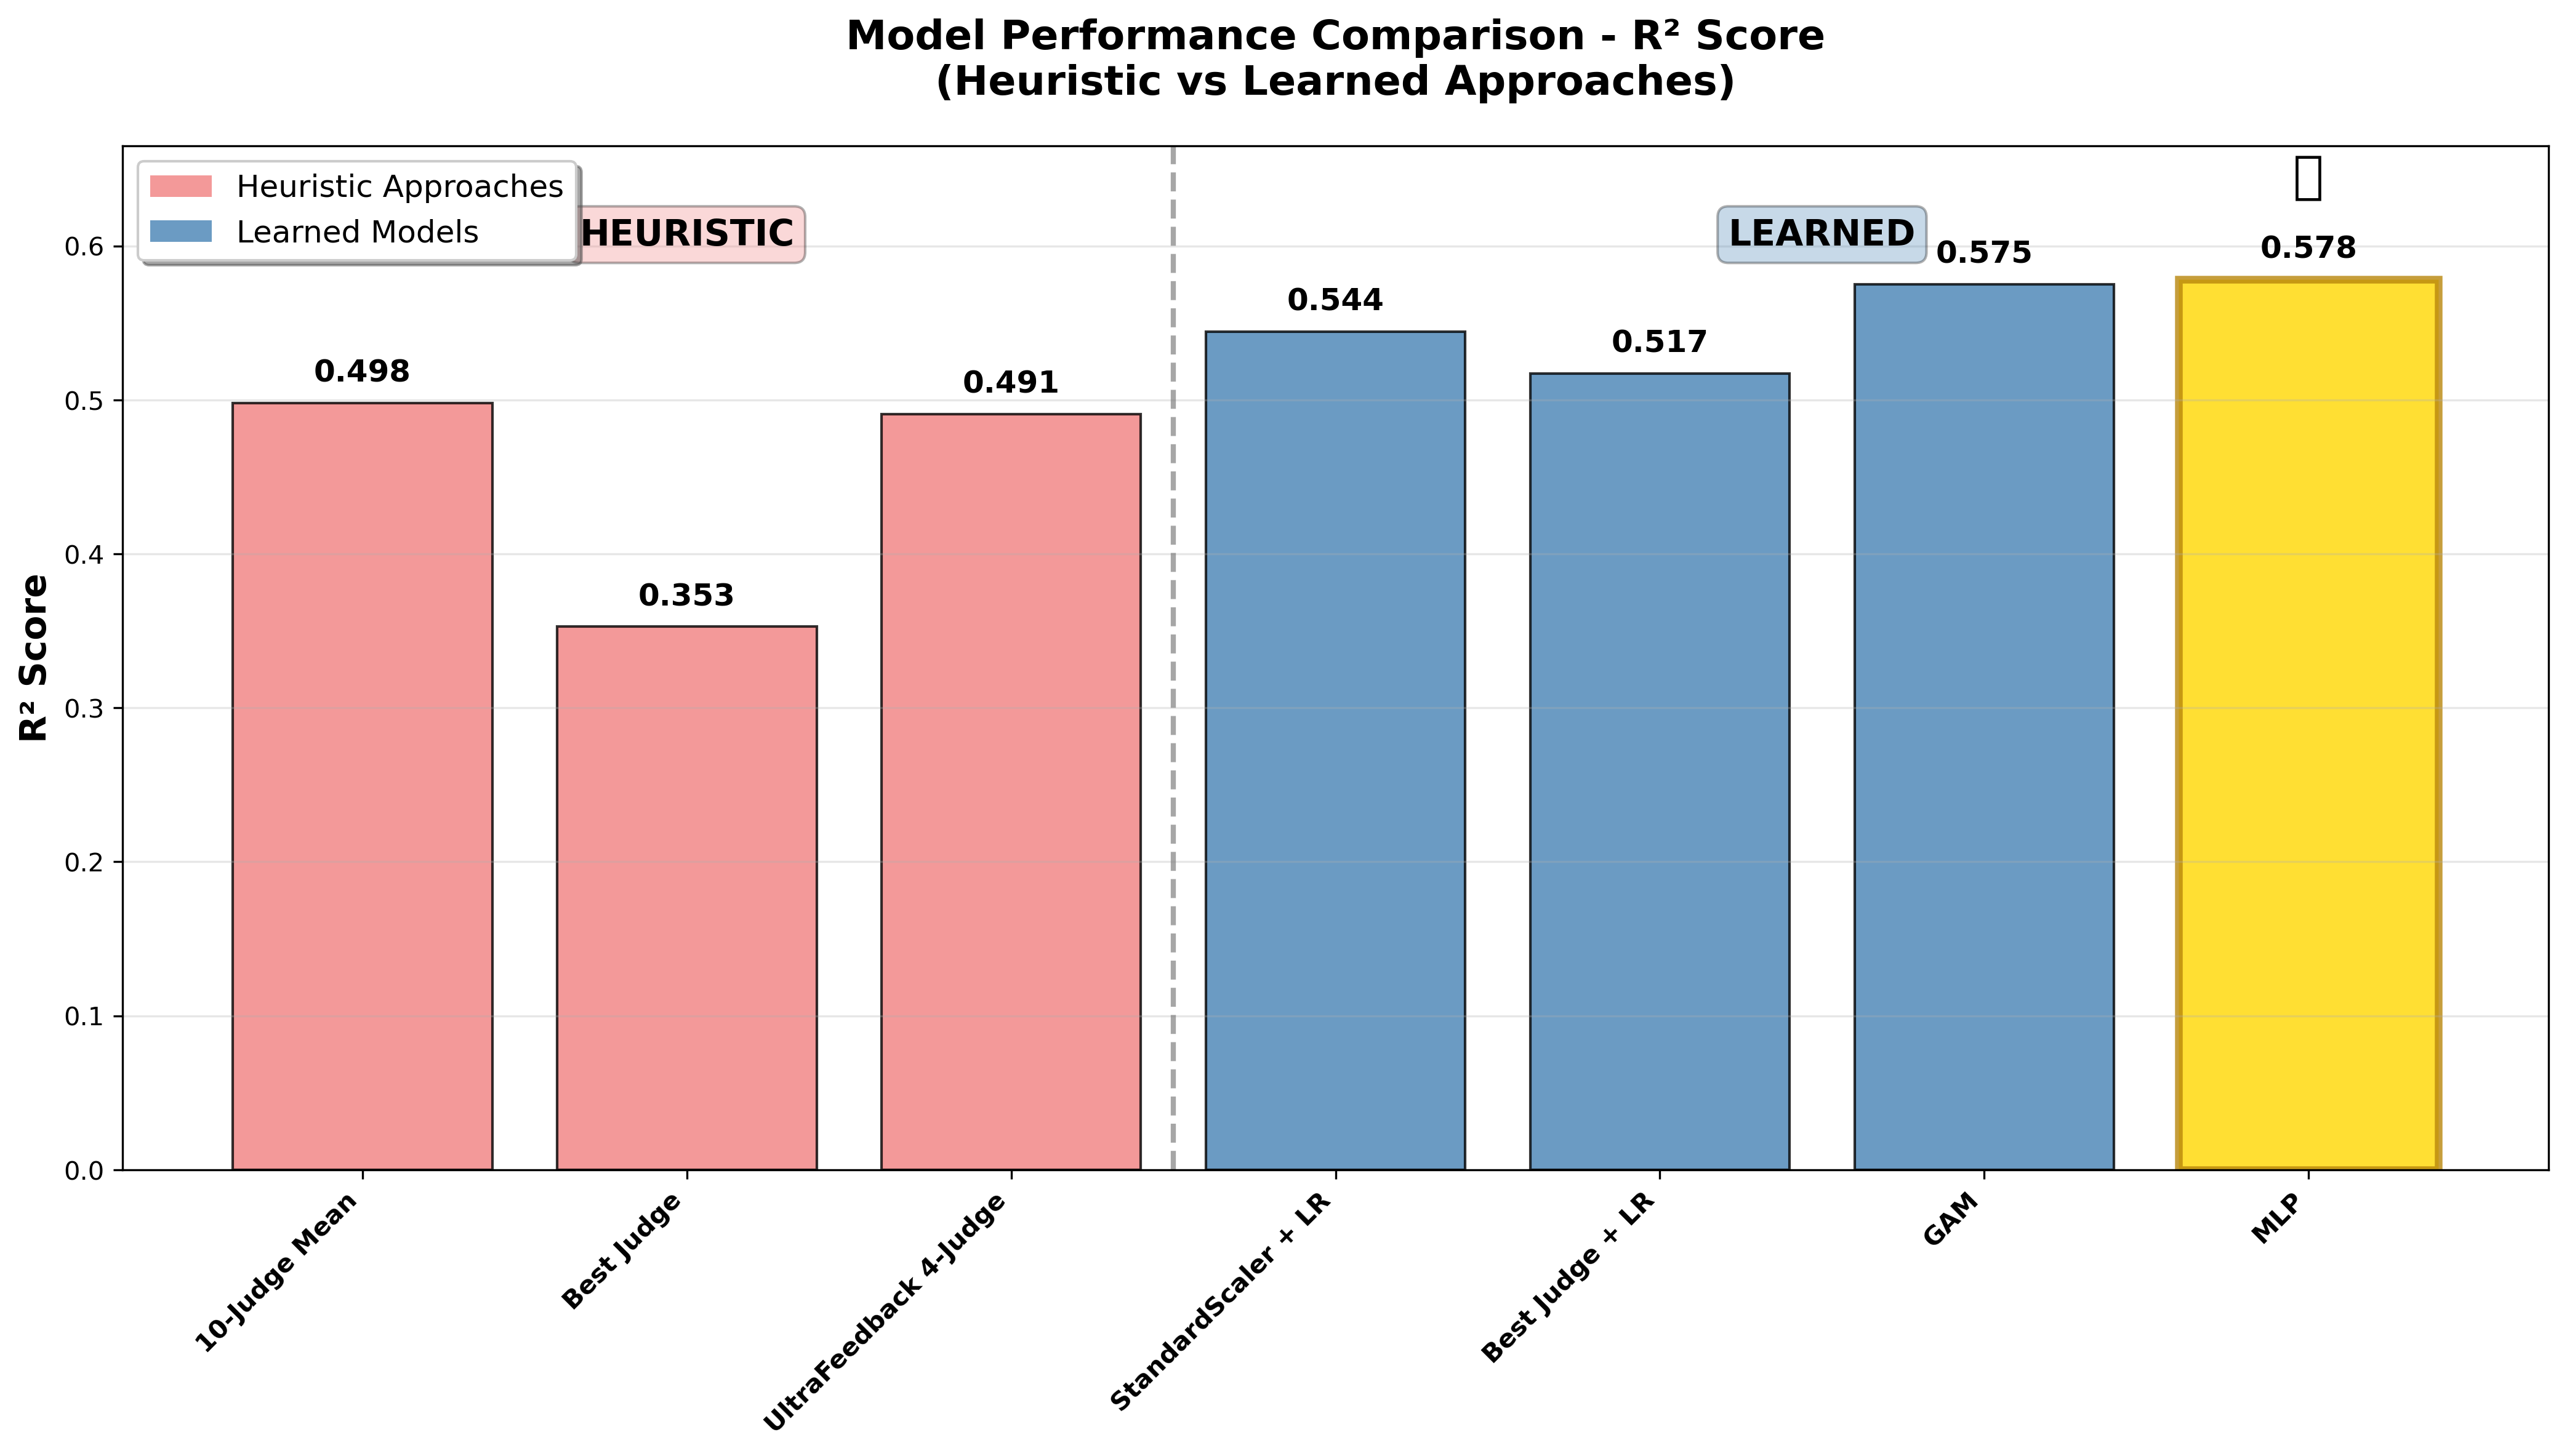
\includegraphics[width=0.5\textwidth]{Result Figures/Main Results/model_comparison.png}
    \caption{Model Performance Comparison: Comprehensive evaluation across all aggregation methods. Our learned approaches (GAM and MLP) substantially outperform all baseline methods. Key results: (1) MLP achieves best overall performance (R² = 0.578), (2) GAM provides comparable performance (R² = 0.575) with full interpretability, (3) Learned linear baselines (R² = 0.544) outperform naive methods, and (4) Single best judge performs significantly worse (R² = 0.353), validating the multi-judge approach.}
    \label{fig:model_comparison}
\end{figure}

\subsection{GAM Analysis: Interpretability and Performance}

Our Generalized Additive Model (GAM) provides highly interpretable judge aggregation with competitive performance. The GAM achieved an R² score of 0.575, demonstrating strong predictive accuracy while maintaining full transparency in how individual judge contributions combine to form final predictions.

THERE ARE SOME UGLY COMMENTED OUT RESULTS HERE. THEY ARE MORE FOR THE APPENDIX, BUT IF YOU'RE CURIOUS...

% \begin{figure}[htbp]
%     \centering
%     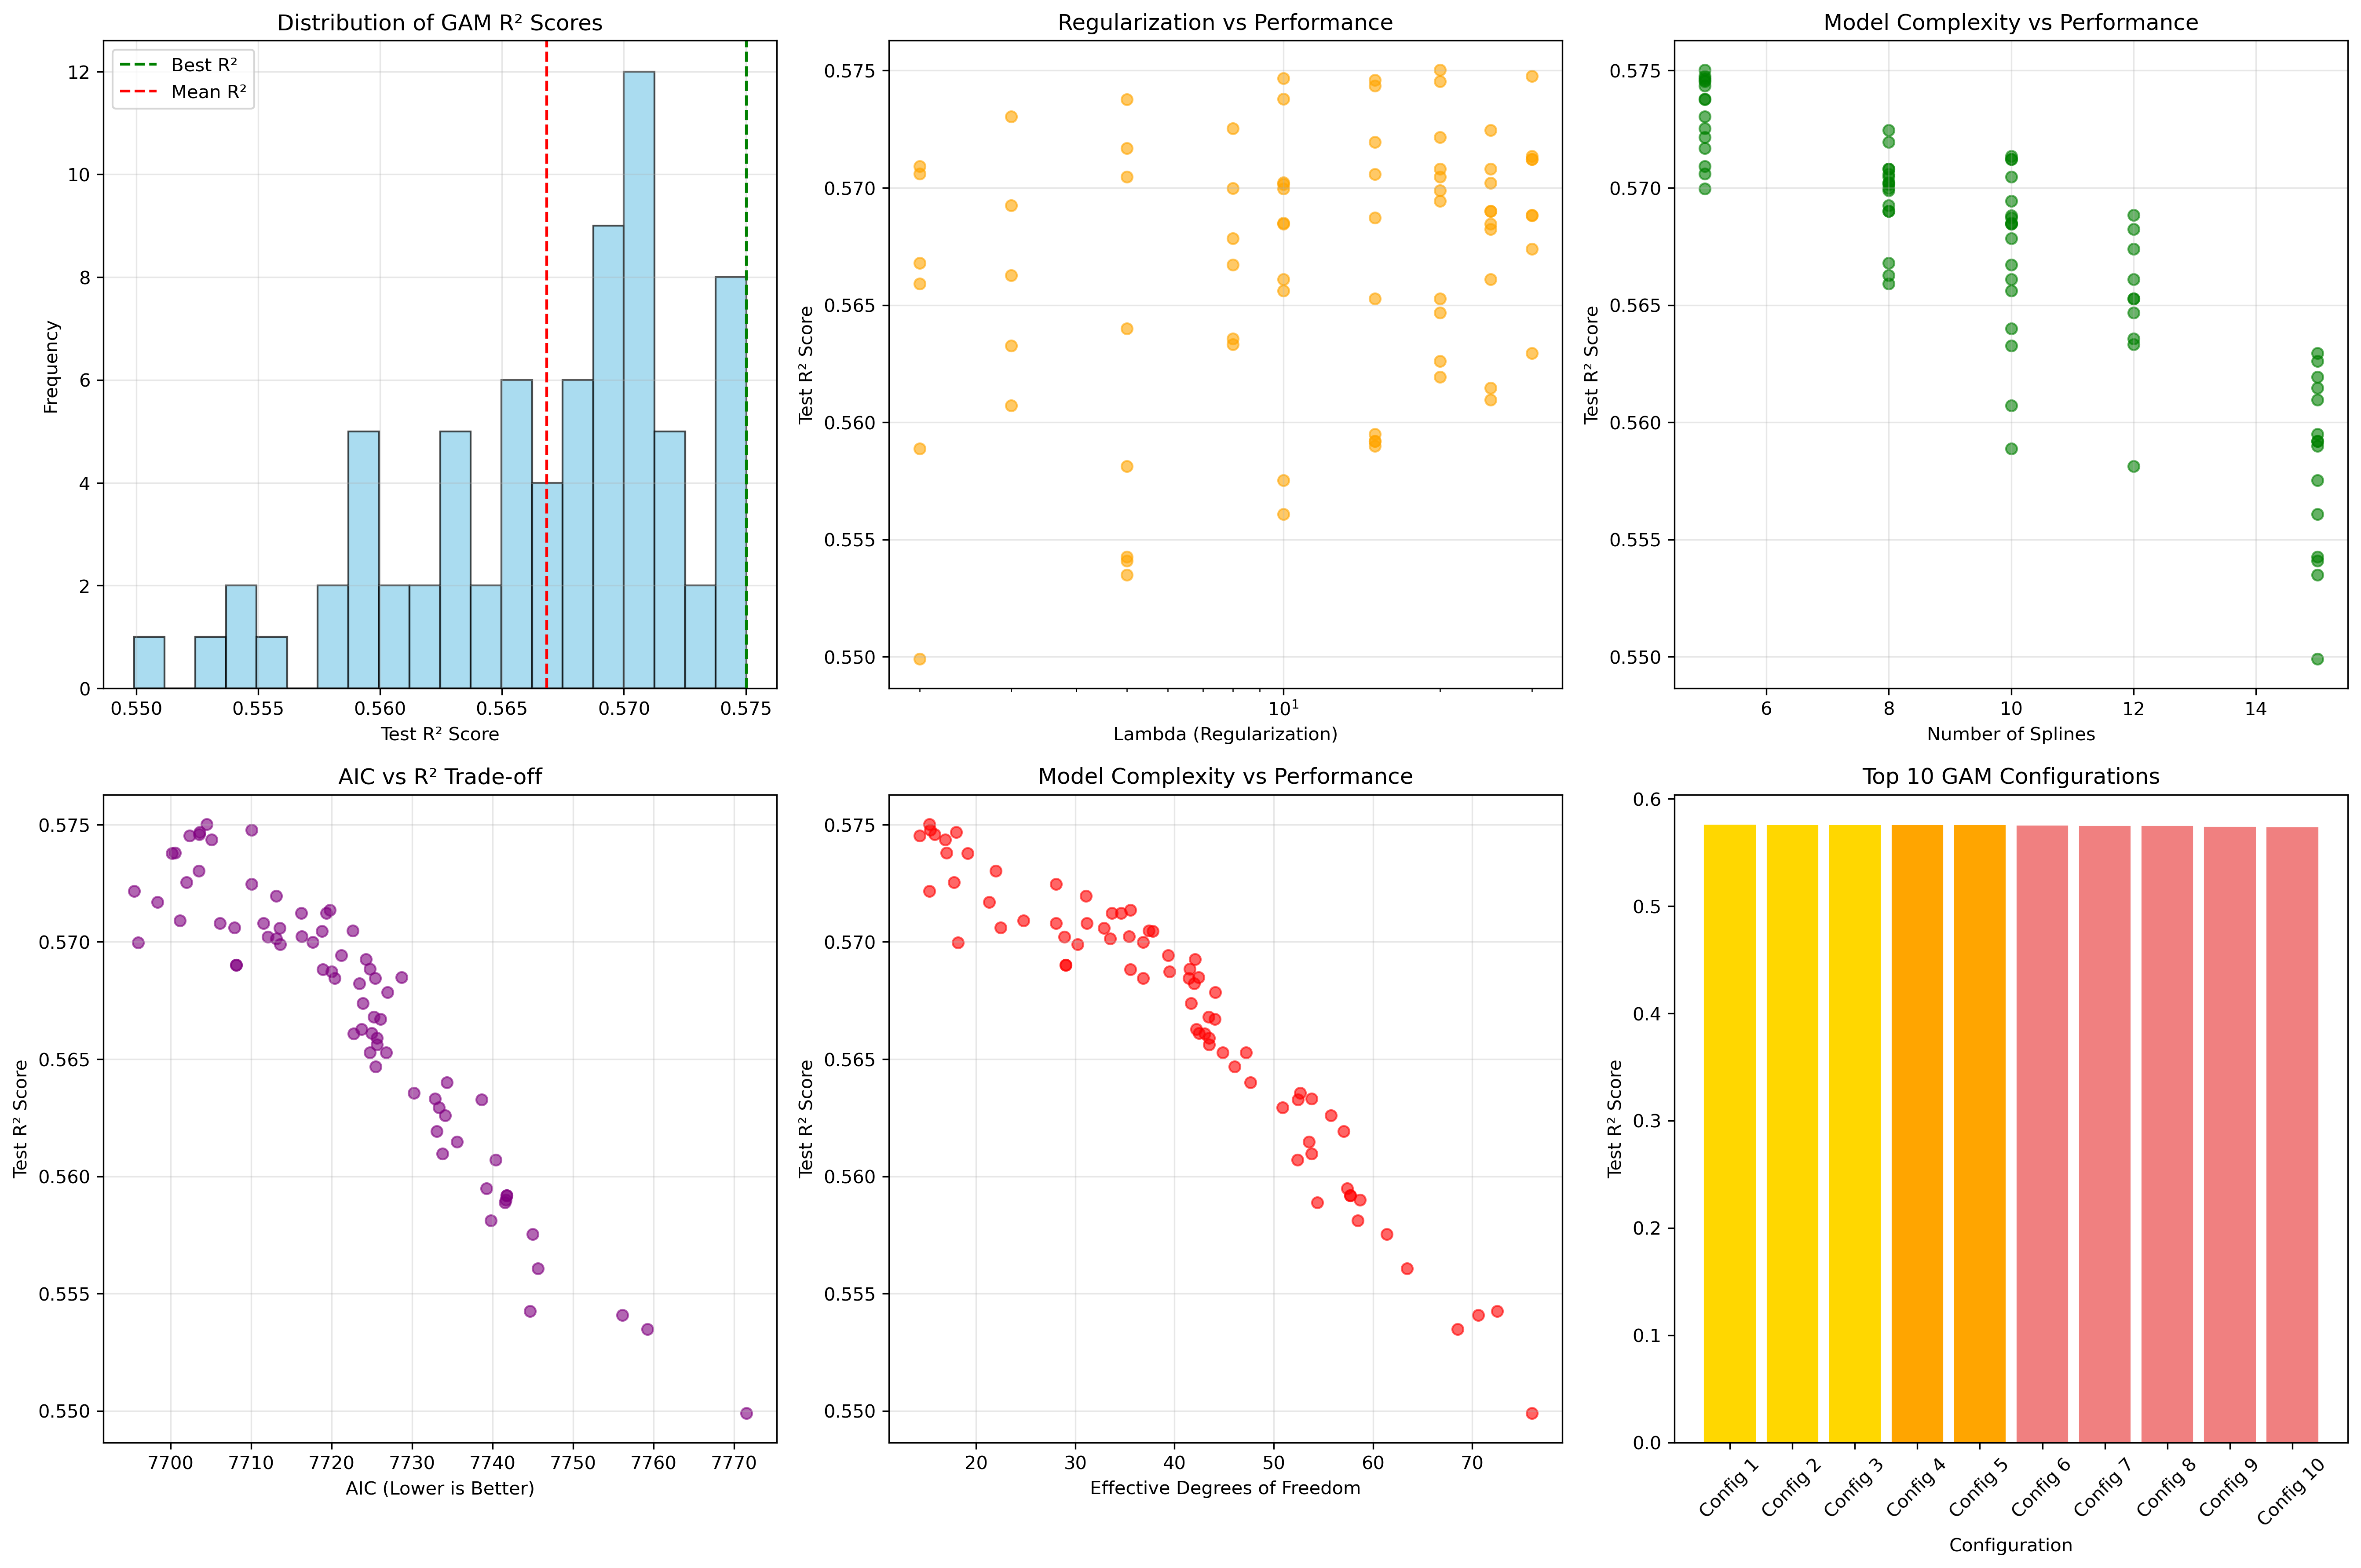
\includegraphics[width=0.5\textwidth]{Result Figures/GAM Analysis/gam_hyperparameter_analysis.png}
%     \caption{GAM Hyperparameter Analysis: Performance surface showing R² scores across different regularization strengths (λ) and spline complexity (n\_splines). The optimal configuration achieves R² = 0.575 with λ = 20.0 and n\_splines = 5, balancing model complexity with interpretability. The analysis shows stable performance across a range of hyperparameters, indicating robust model behavior.}
%     \label{fig:gam_hyperparameter_analysis}
% \end{figure}

% \begin{figure}[htbp]
%     \centering
%     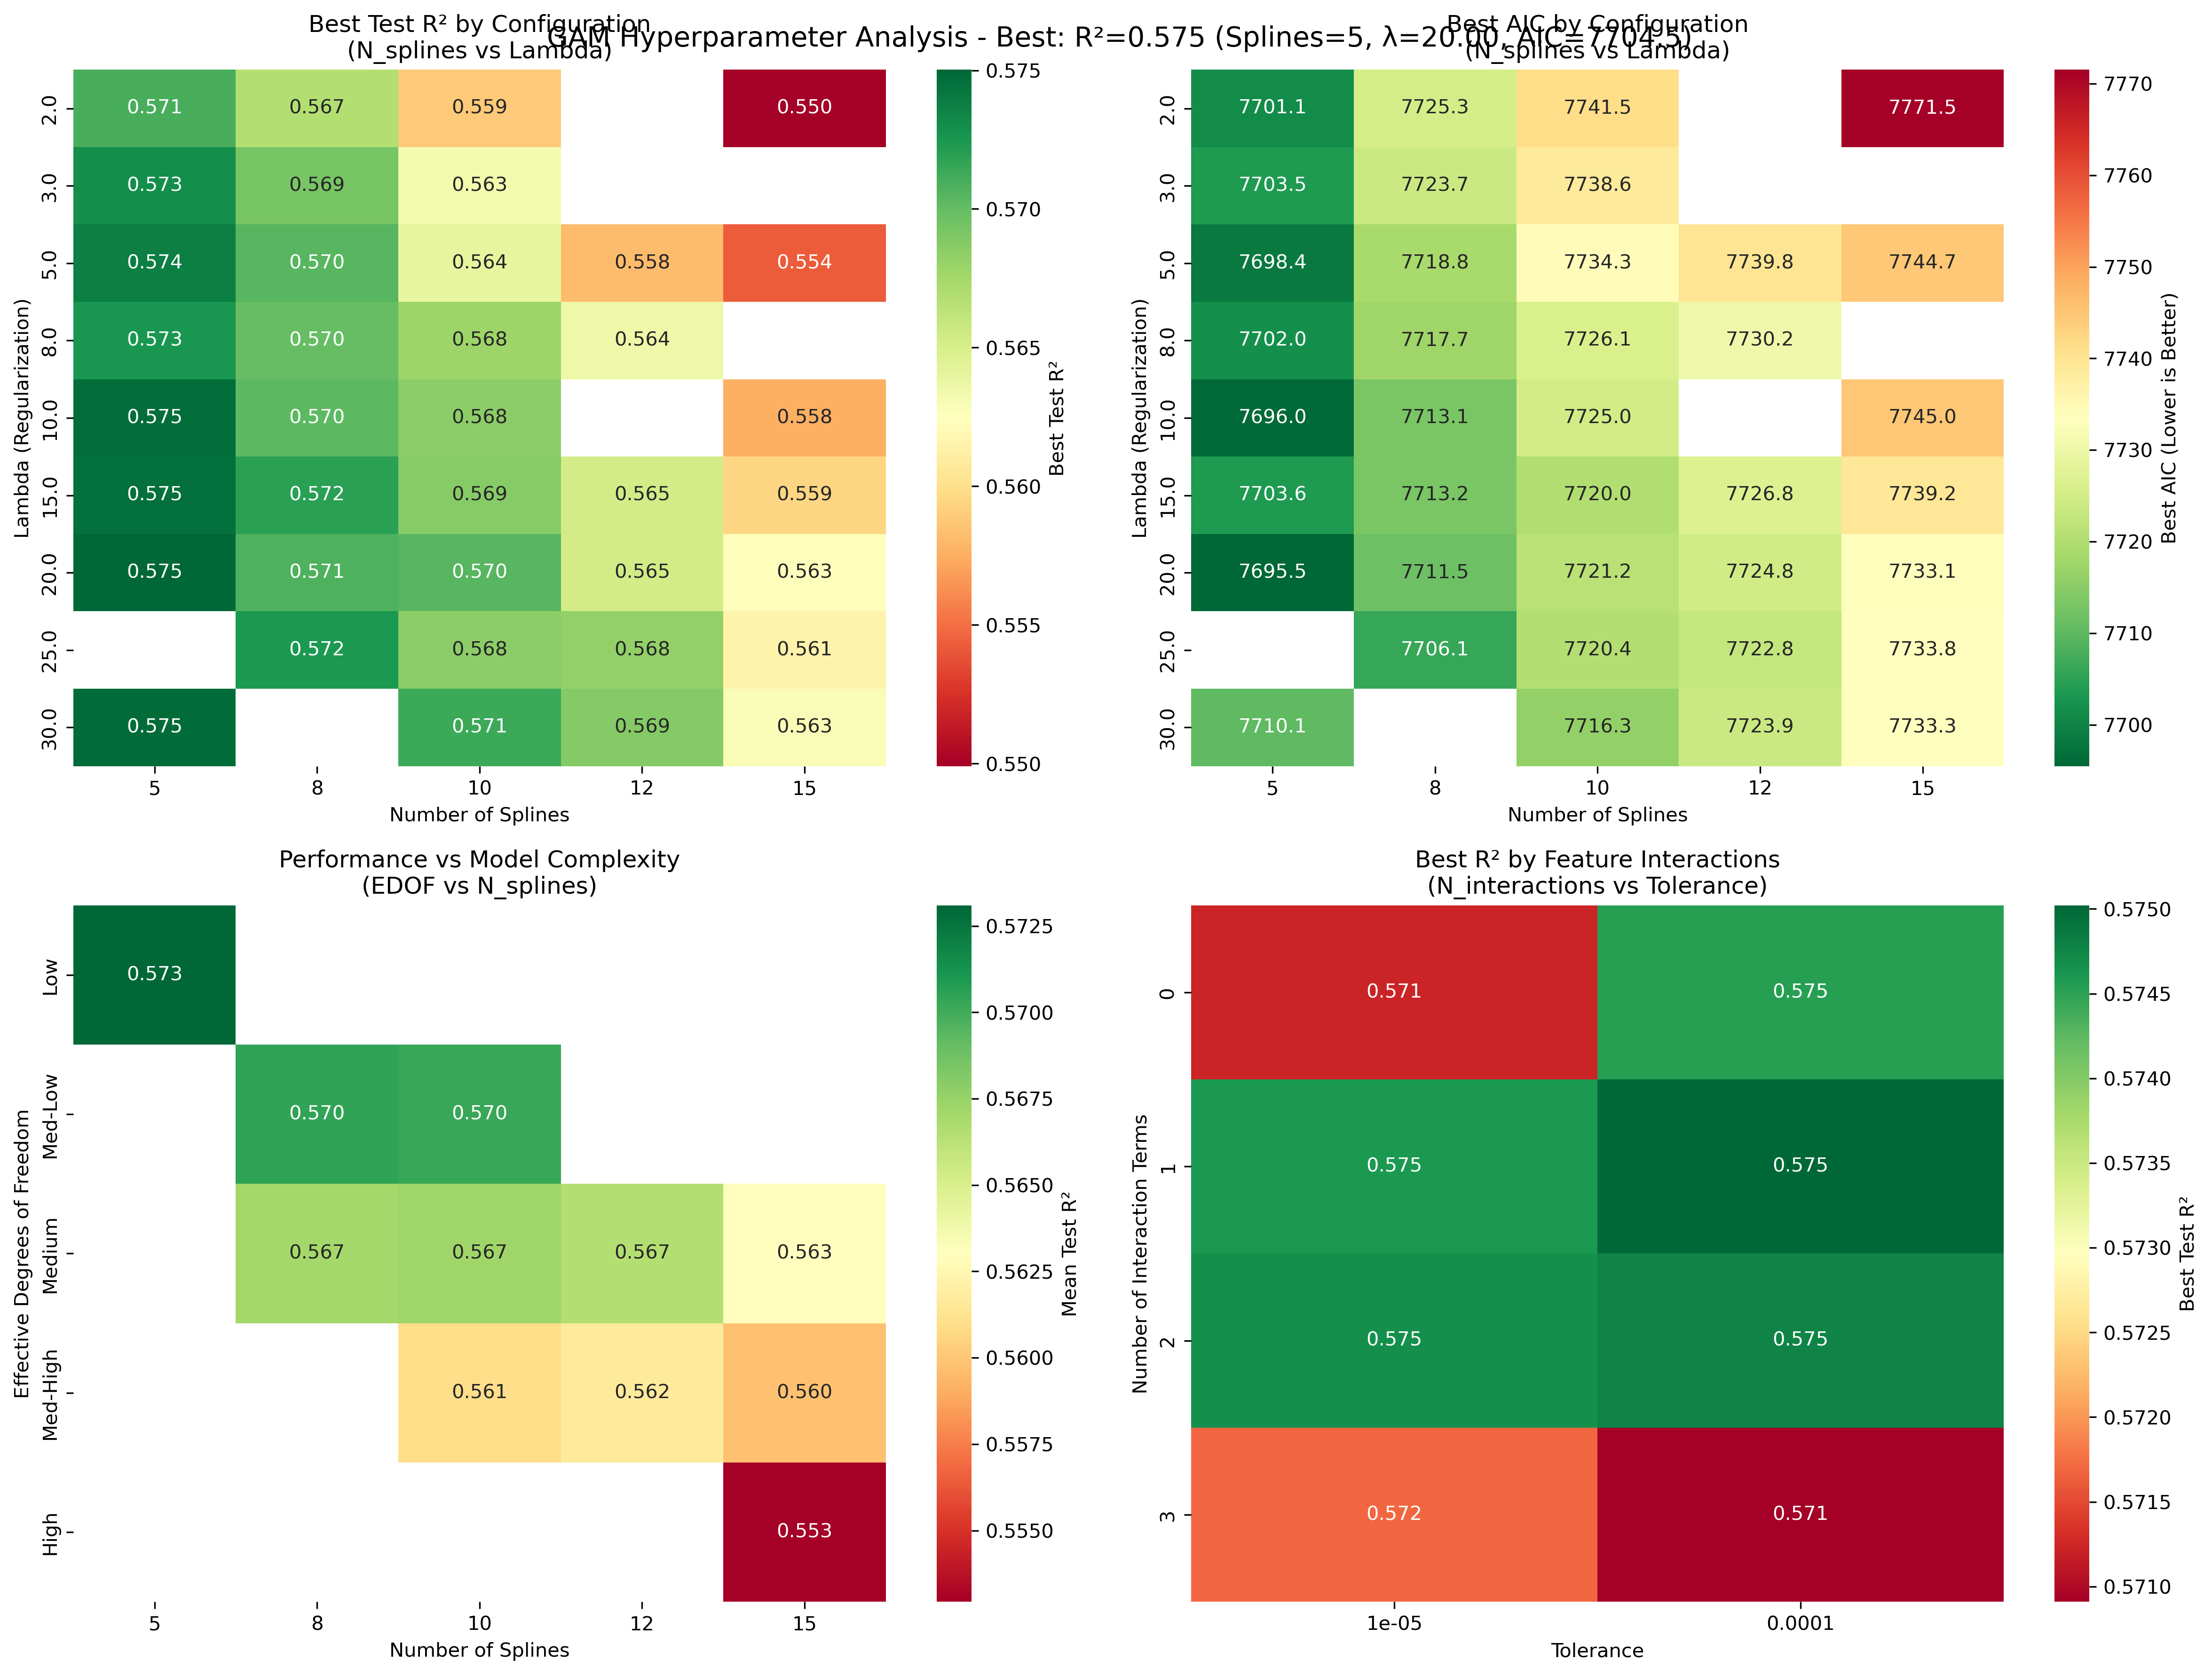
\includegraphics[width=0.5\textwidth]{Result Figures/GAM Analysis/gam_hyperparameter_heatmap.png}
%     \caption{GAM Hyperparameter Heatmap: Detailed performance matrix across hyperparameter space. Darker regions indicate higher R² scores. The optimal region shows λ values between 10-30 work well with moderate spline complexity (3-7 splines), providing a practical guide for hyperparameter selection in similar multi-judge aggregation tasks.}
%     \label{fig:gam_hyperparameter_heatmap}
% \end{figure}

% \begin{figure}[htbp]
%     \centering
%     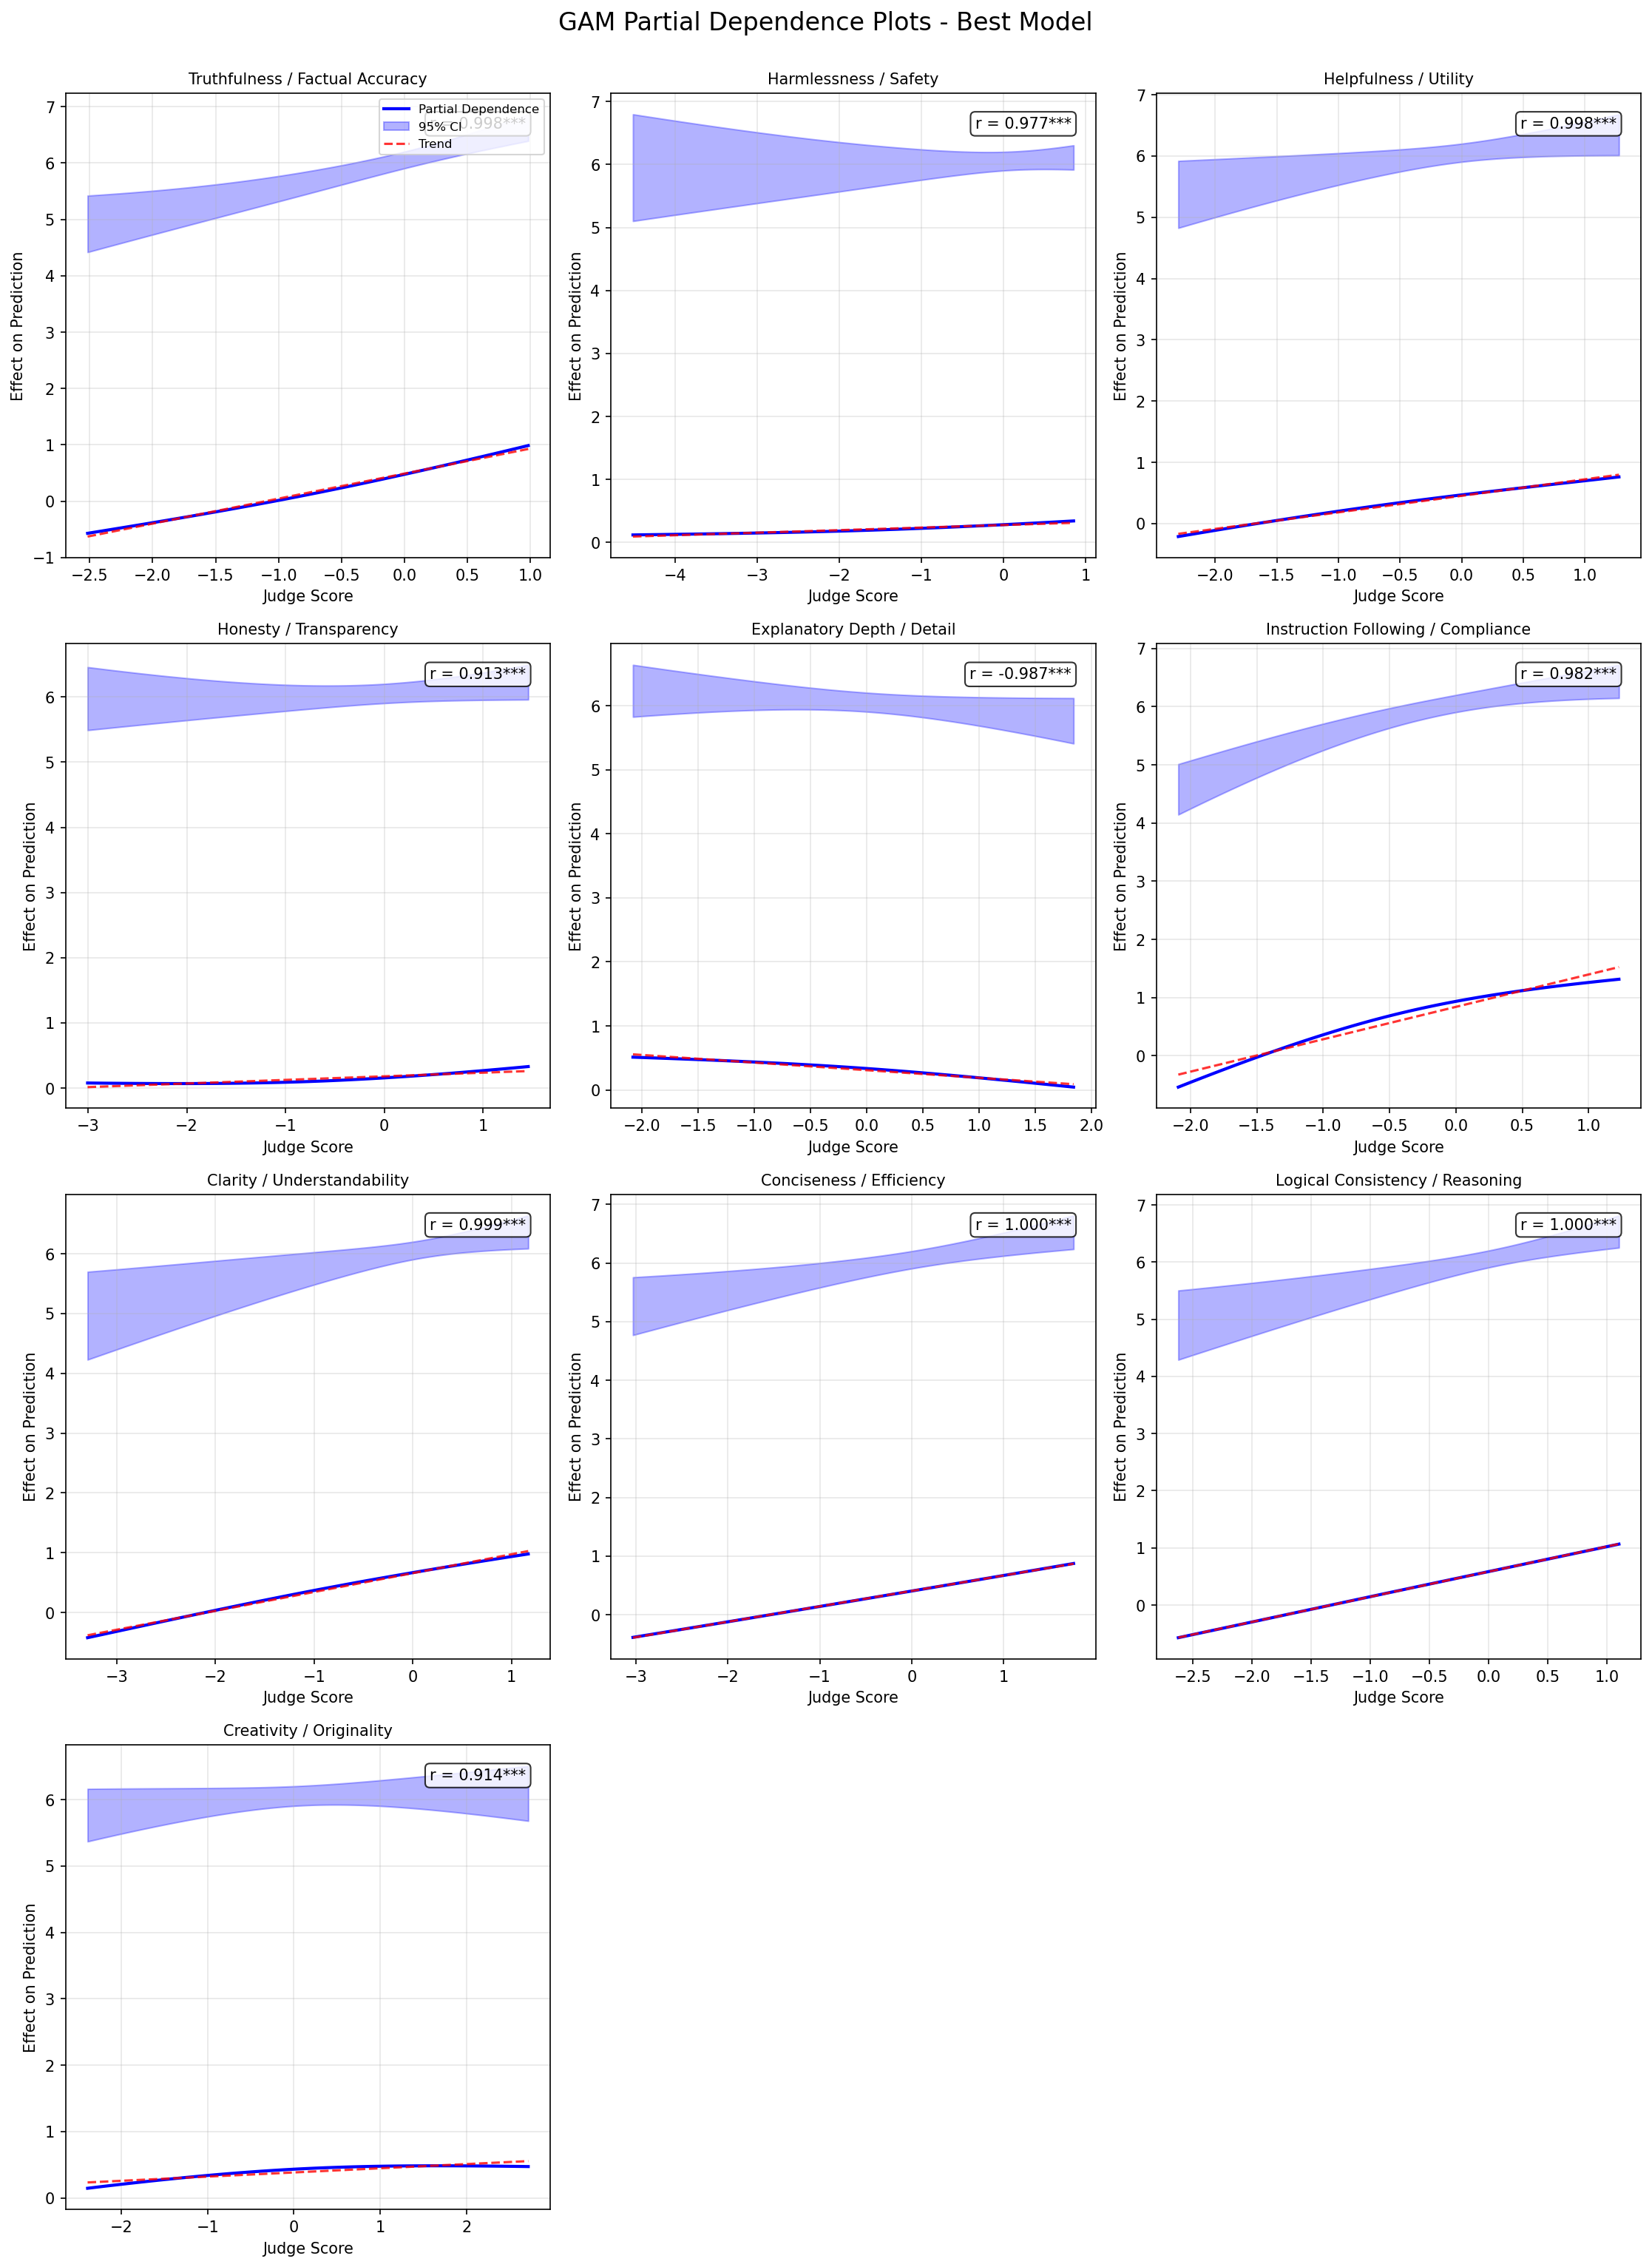
\includegraphics[width=0.5\textwidth]{Result Figures/GAM Analysis/gam_partial_dependence_plots.png}
%     \caption{GAM Partial Dependence Plots: Individual judge contribution patterns showing how each specialized judge influences the final prediction. Key findings: (1) Instruction Following and Truthfulness show near-linear positive relationships, (2) Logical Consistency demonstrates the strongest monotonic contribution, (3) Harmlessness exhibits non-linear effects with threshold behavior, and (4) Some judges show interaction effects, particularly between Truthfulness and Helpfulness dimensions.}
%     \label{fig:gam_partial_dependence}
% \end{figure}

\begin{figure}[htbp]
    \centering
    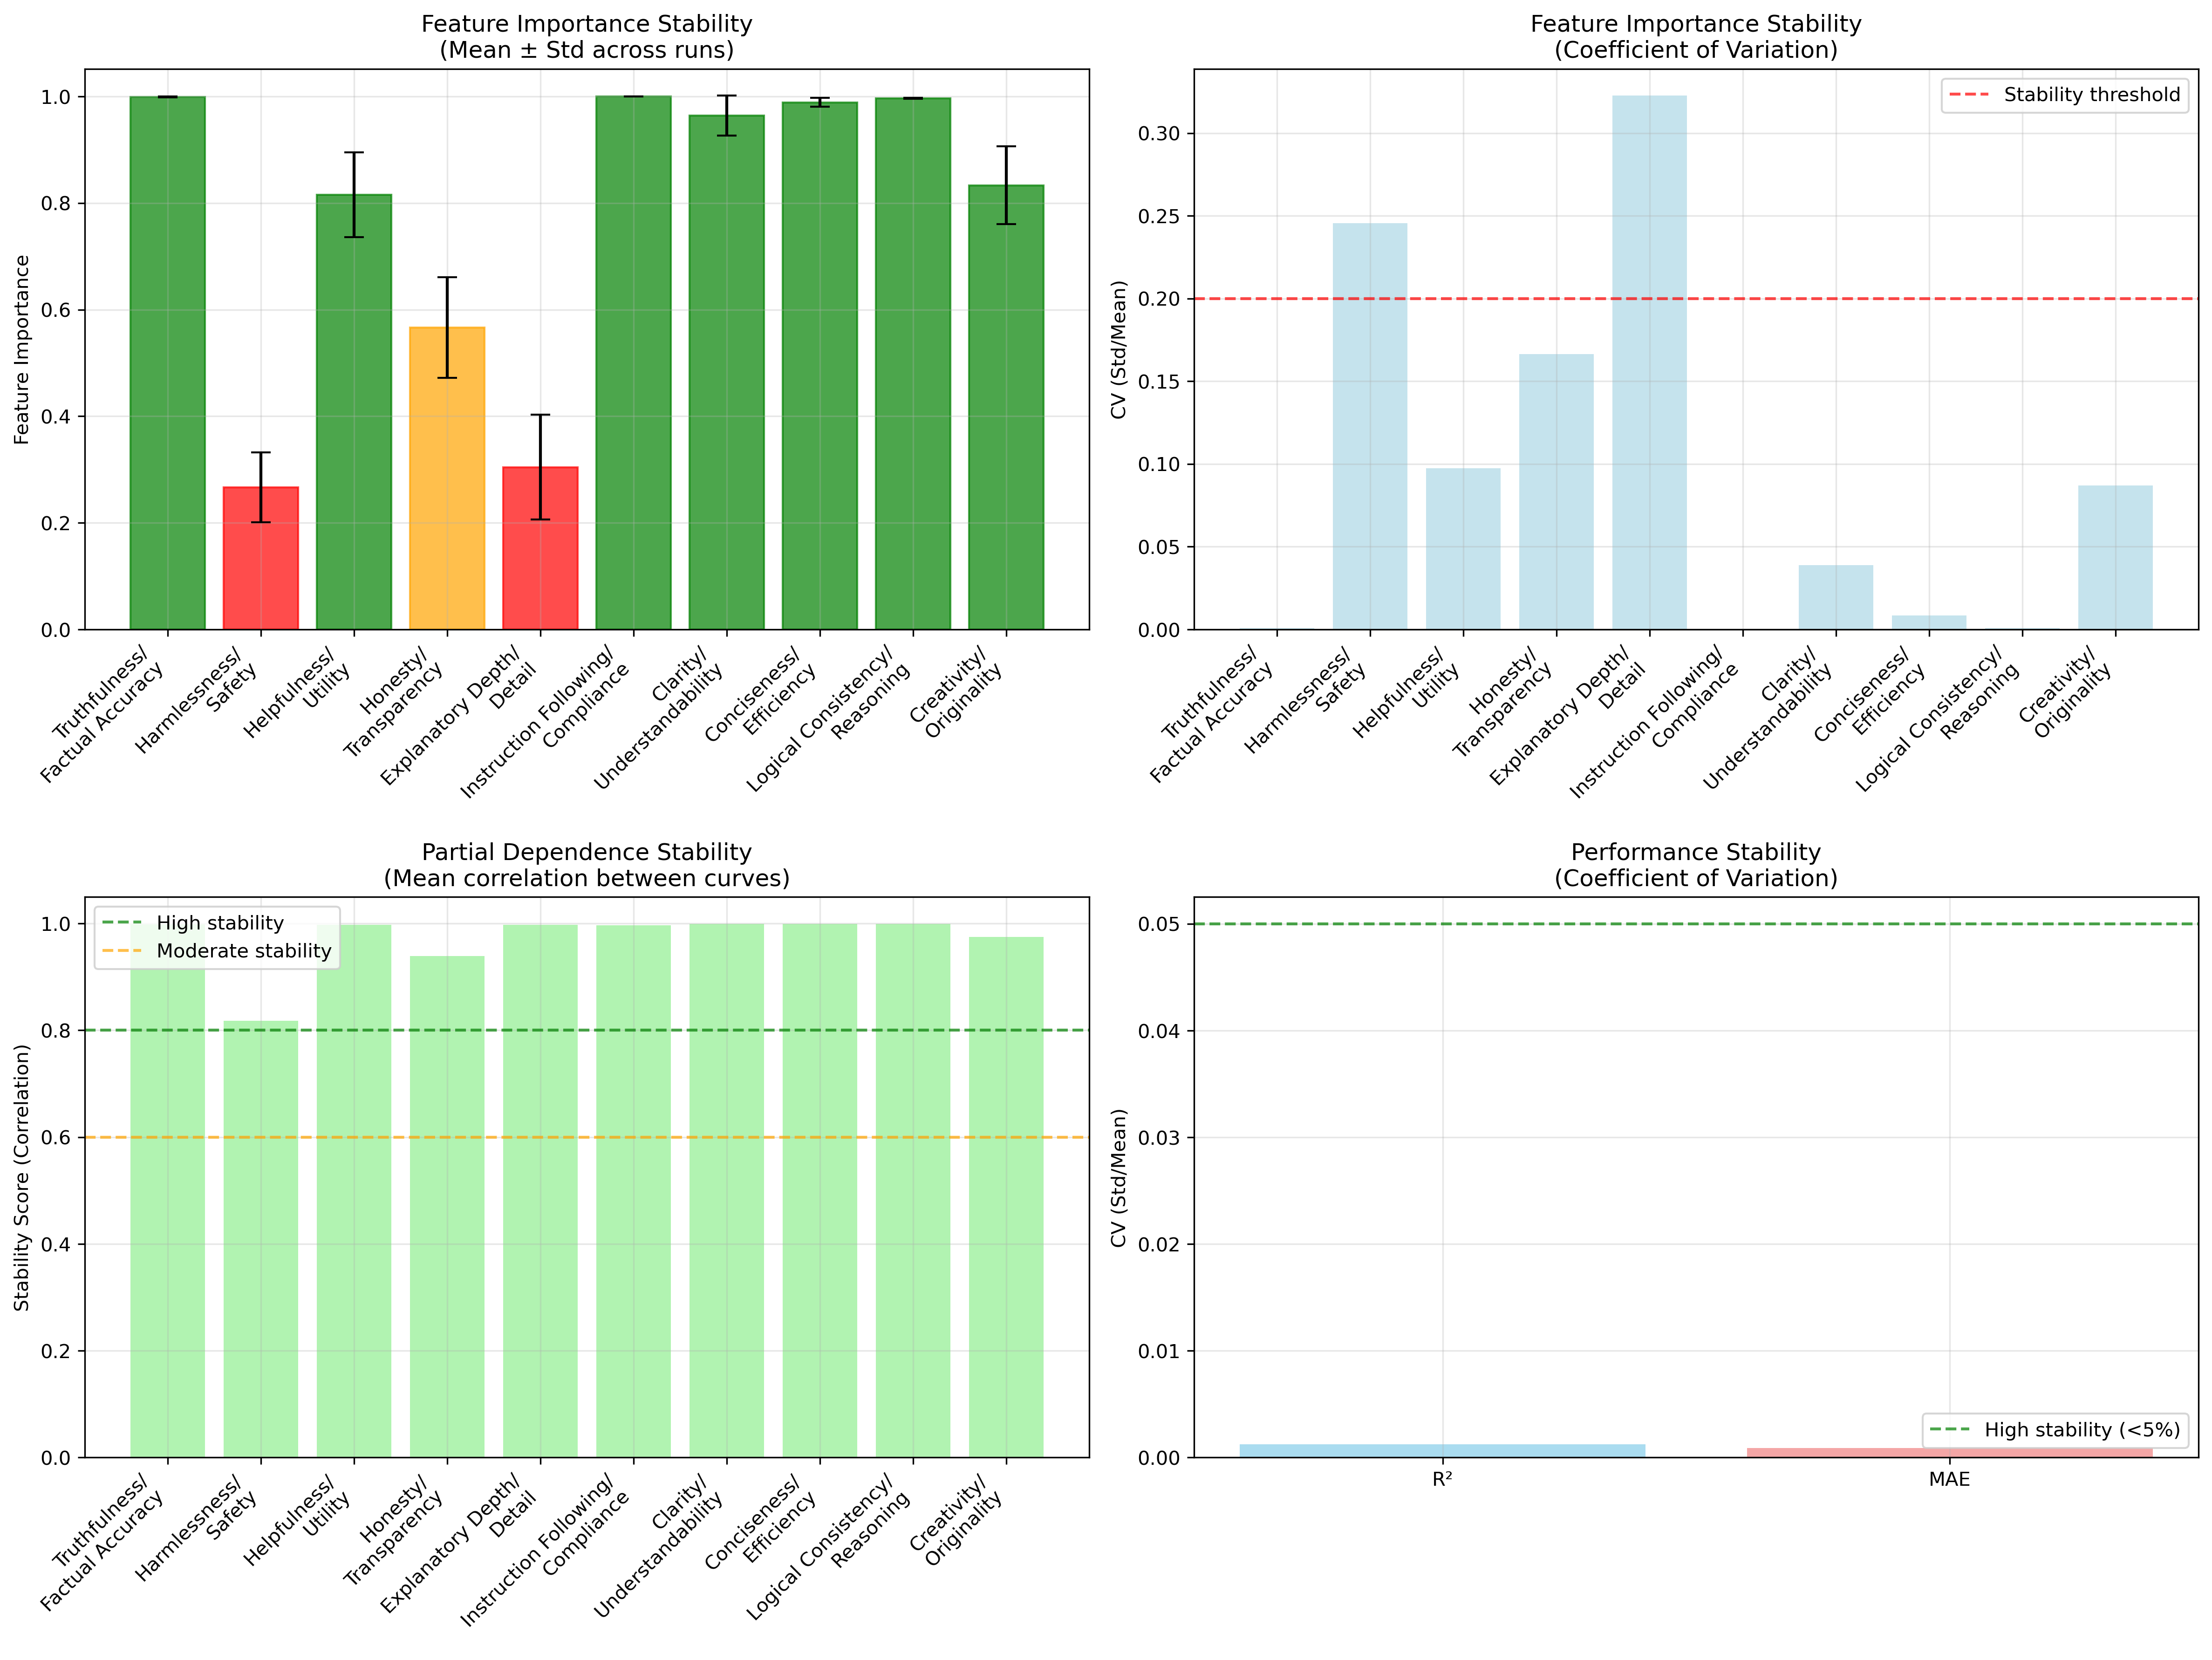
\includegraphics[width=0.5\textwidth]{Result Figures/GAM Analysis/gam_stability_analysis.png}
    \caption{GAM Stability Analysis: Feature importance consistency across 20 independent model training runs. The analysis demonstrates that our GAM produces stable and reproducible feature importance rankings, with Truthfulness, Instruction Following, and Logical Consistency consistently ranking as top contributors. Low variance in importance scores (error bars) indicates reliable interpretability across different training initializations.}
    \label{fig:gam_stability}
\end{figure}

\subsection{Case Study: System Robustness}

In the following section, we evaluate our aggregator's robustness to:
\begin{itemize}
    \item Biases in the human preference data.
    \item Biases in the judges.
\end{itemize}

For the first case, we don't compare with any baselines, as the naive methods are not trained with human feedback data, so their bias wouldn't affect their scores on the \textbf{true preferences}. On the second case however, we compare with the \textit{Naive Mean} baseline, given that it uses the judges scores to predict the human preferences.


\subsubsection{Persona Contamination Analysis: Robustness to Human Biases}

We evaluate system robustness under three contamination strategies, each representing different real-world scenarios: (1) \textbf{Systematic bias} - humans consistently shift scores in one direction [Note: this is relevant, for example, as we see different cultures give consistently higher or lower scores in general], (2) \textbf{Random noise} - humans provide completely random preference scores, representing either random responses or severely broken preference criteria, and (3) \textbf{Scaled-down} contamination - some humans systematically undervalue all responses.

\textbf{Additional robustness experiments pending:} We are currently finalizing results on judge contamination robustness (testing with deliberately compromised individual judges).

\begin{figure}[htbp]
    \centering
    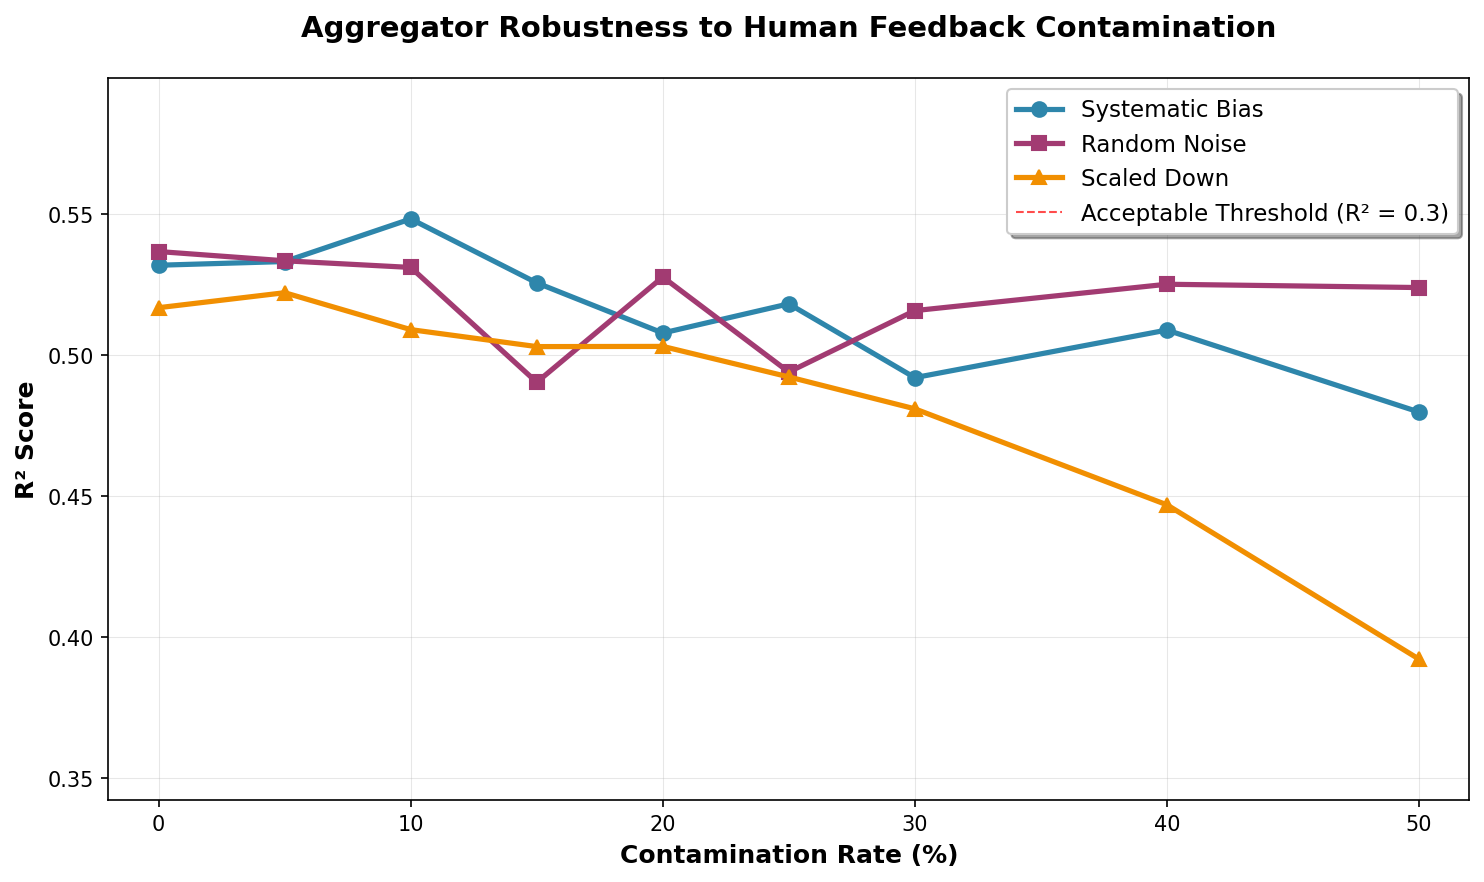
\includegraphics[width=0.5\textwidth]{Result Figures/Robustness Results/persona_robustness/aggregator_robustness_analysis.png}
    \caption{Aggregator Robustness Analysis: Performance degradation under different contamination strategies across contamination rates from 0\% to 50\%. Key findings: (1) \textbf{Systematic bias} shows gradual degradation with performance dropping from R² = 0.532 to R² = 0.480 at 50\% contamination, (2) \textbf{Random noise} maintains relatively stable performance until 15\% contamination, then shows moderate decline, and (3) \textbf{Scaled-down} contamination causes the most severe degradation, with R² dropping to 0.392 at 50\% contamination. The system demonstrates reasonable robustness up to 20\% contamination across all strategies, supporting deployment in environments with moderate human preference score contamination.}
    \label{fig:robustness_analysis}
\end{figure}

\subsubsection{Rubric Sensitivity Analysis: Judge Robustness to Scoring Variations}

We evaluate how sensitive our aggregation models are to variations in judge rubric formulations, testing whether learned models maintain their advantages when judge evaluation criteria are modified. This modifications are simulated by applying different bias transformations to the scores of the judges. The results show that the learned models are robust to these variations, while the naive mean method is not.

\begin{figure}[H]
    \centering
    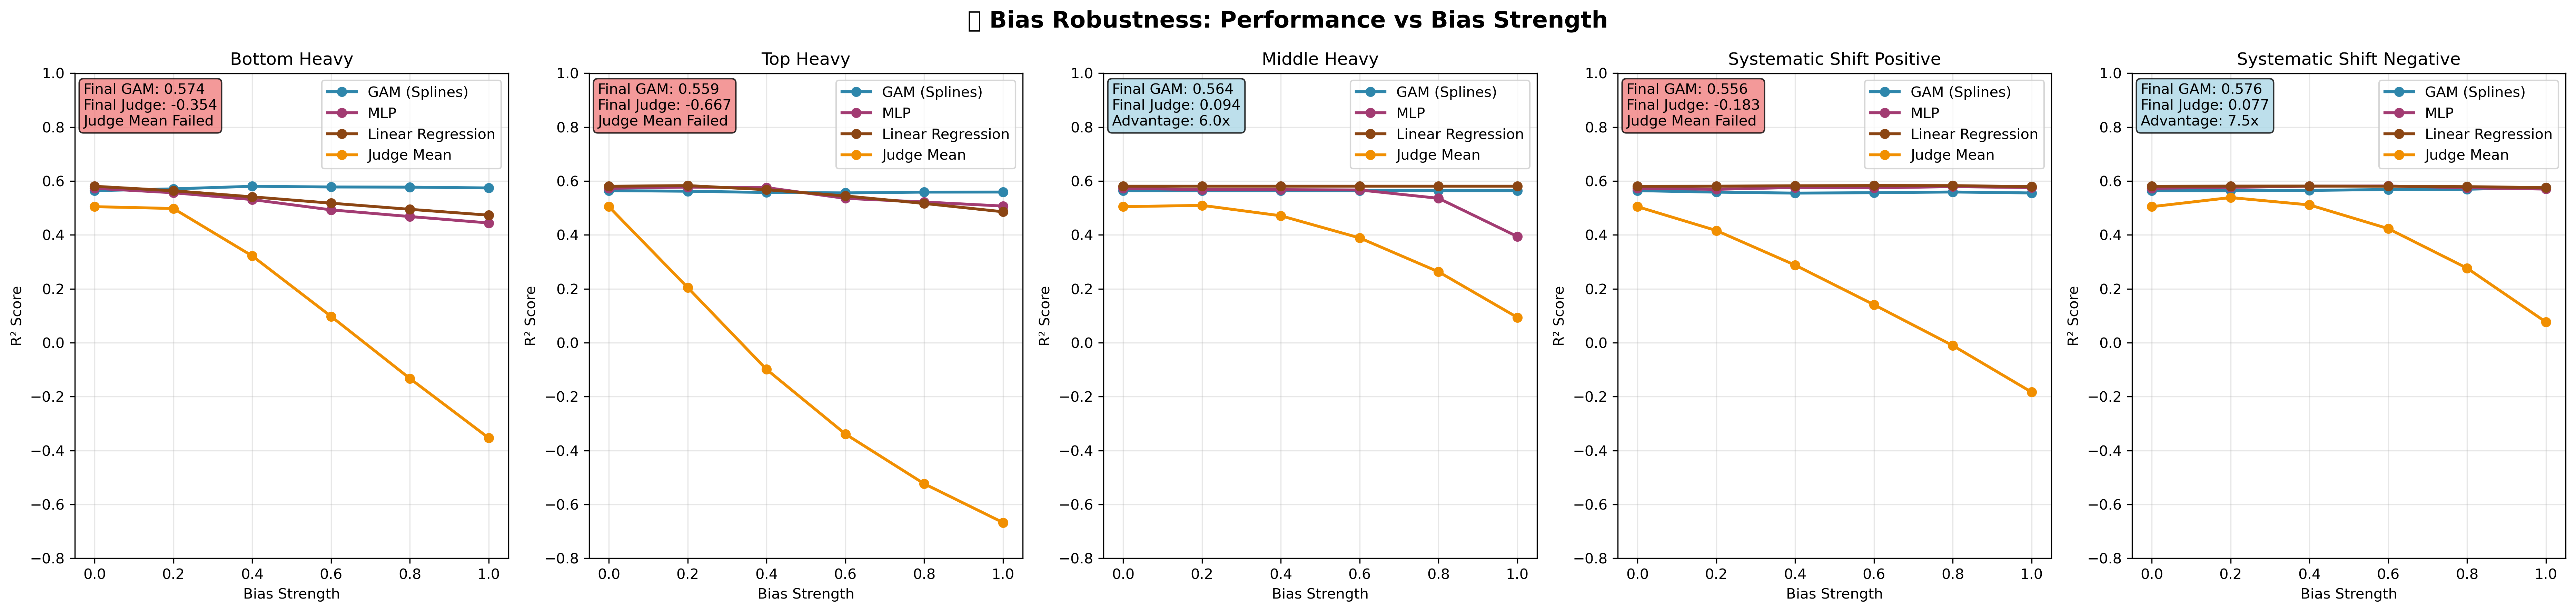
\includegraphics[width=0.8\textwidth]{Result Figures/Rubric Sensitivity/bias_robustness_analysis.png}
    \caption{Bias Robustness Analysis: Performance comparison across different bias transformation types and strengths. The analysis shows five bias scenarios: Bottom Heavy, Top Heavy, Middle Heavy, Systematic Shift Positive, and Systematic Shift Negative. \textbf{Simple Judge Mean} (orange) shows dramatic performance degradation under bias, dropping to negative R² values, while \textbf{Learned models} (GAM, MLP, Linear Regression) maintain stable performance across most bias types, with GAM and MLP showing superior robustness.}
    \label{fig:bias_robustness}
\end{figure}

\begin{figure}[H]
    \centering
    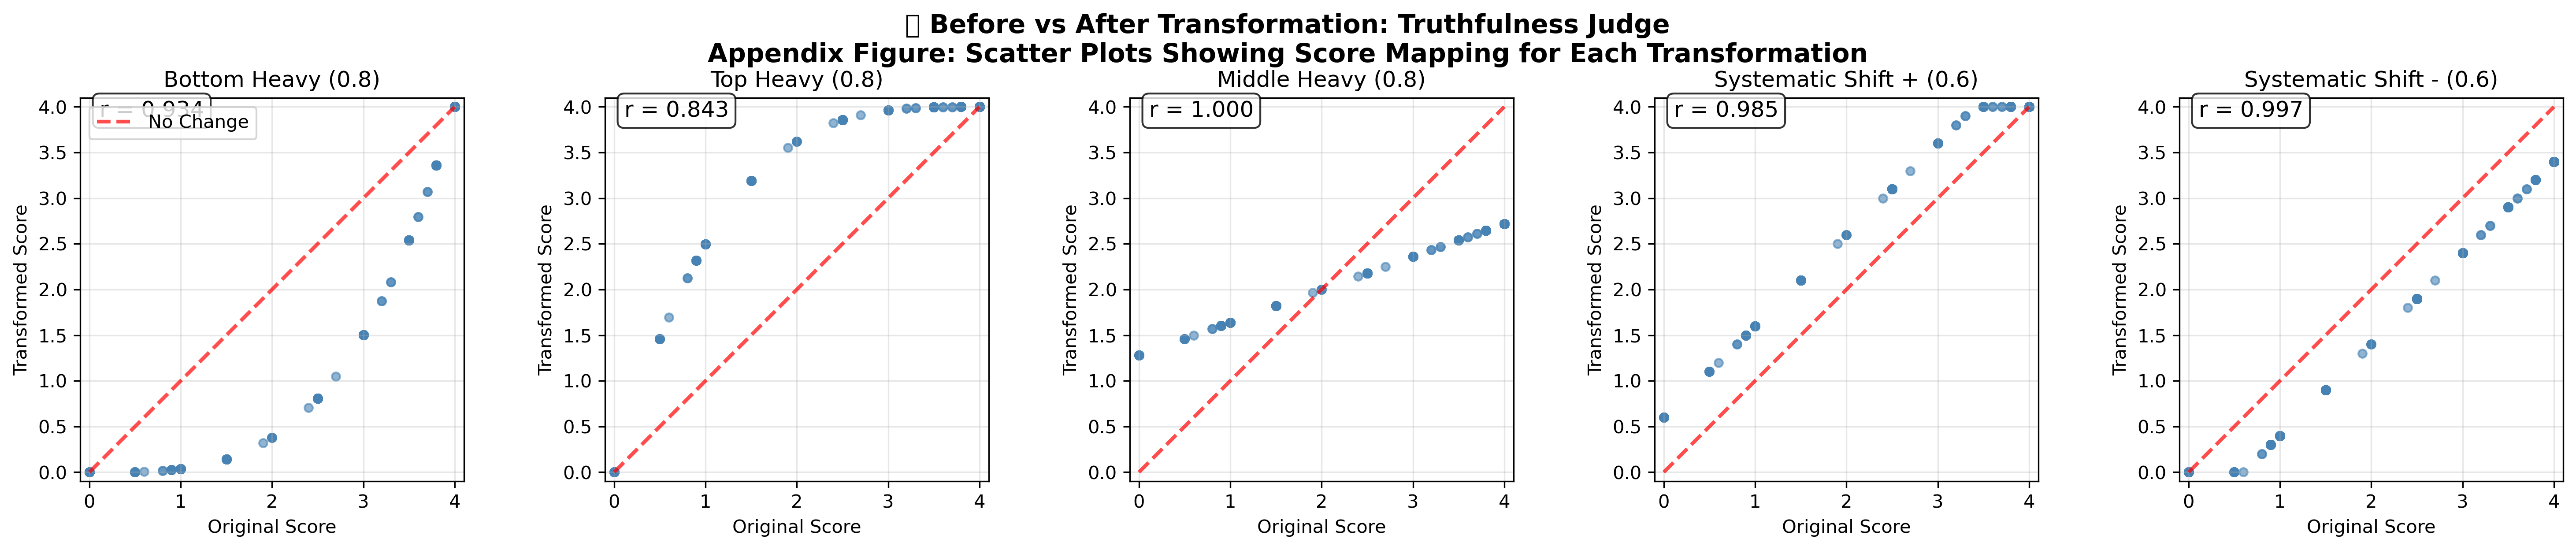
\includegraphics[width=0.8\textwidth]{Result Figures/Rubric Sensitivity/transformation_scatter_plots_appendix.png}
    \caption{Transformation Scatter Plots: Score mapping relationships for the Truthfulness judge under different bias transformations. Each panel shows original scores (x-axis) vs. transformed scores (y-axis) with correlation coefficients. The transformation strength that was applied is reported in the title of each panel.}
    \label{fig:transformation_scatter}
\end{figure}

\subsection{Methodology Validation: Is Diverse Persona Sampling Limiting Performance?}

A critical question for our framework is whether the relatively modest aggregator performance (R² ≈ 0.55) reflects fundamental limitations of our approach, or whether it stems from our methodological choice to sample ground truth from highly diverse personas with conflicting preference profiles. Our baseline approach uniformly samples across 14 distinct personas—from Child to Professor to CEO—creating inherently high-variance ground truth that may be artificially constraining what any aggregation model can achieve.

To test whether our diverse persona sampling methodology is limiting aggregator performance, we conducted a controlled comparison across four ground truth conditions: (1) Mixed personas (our baseline diverse sampling), (2) UltraFeedback GPT-4 generated scores (consistent single-model preferences), (3) Individual persona preferences (internally consistent but narrow profiles), and (4) Mathematical average of all personas (preserving diversity signal while reducing sampling noise). This systematic evaluation isolates the impact of preference diversity on aggregation performance, testing whether more consistent ground truth would reveal superior aggregator capabilities masked by our diverse sampling strategy.

\begin{figure}[htbp]
    \centering
    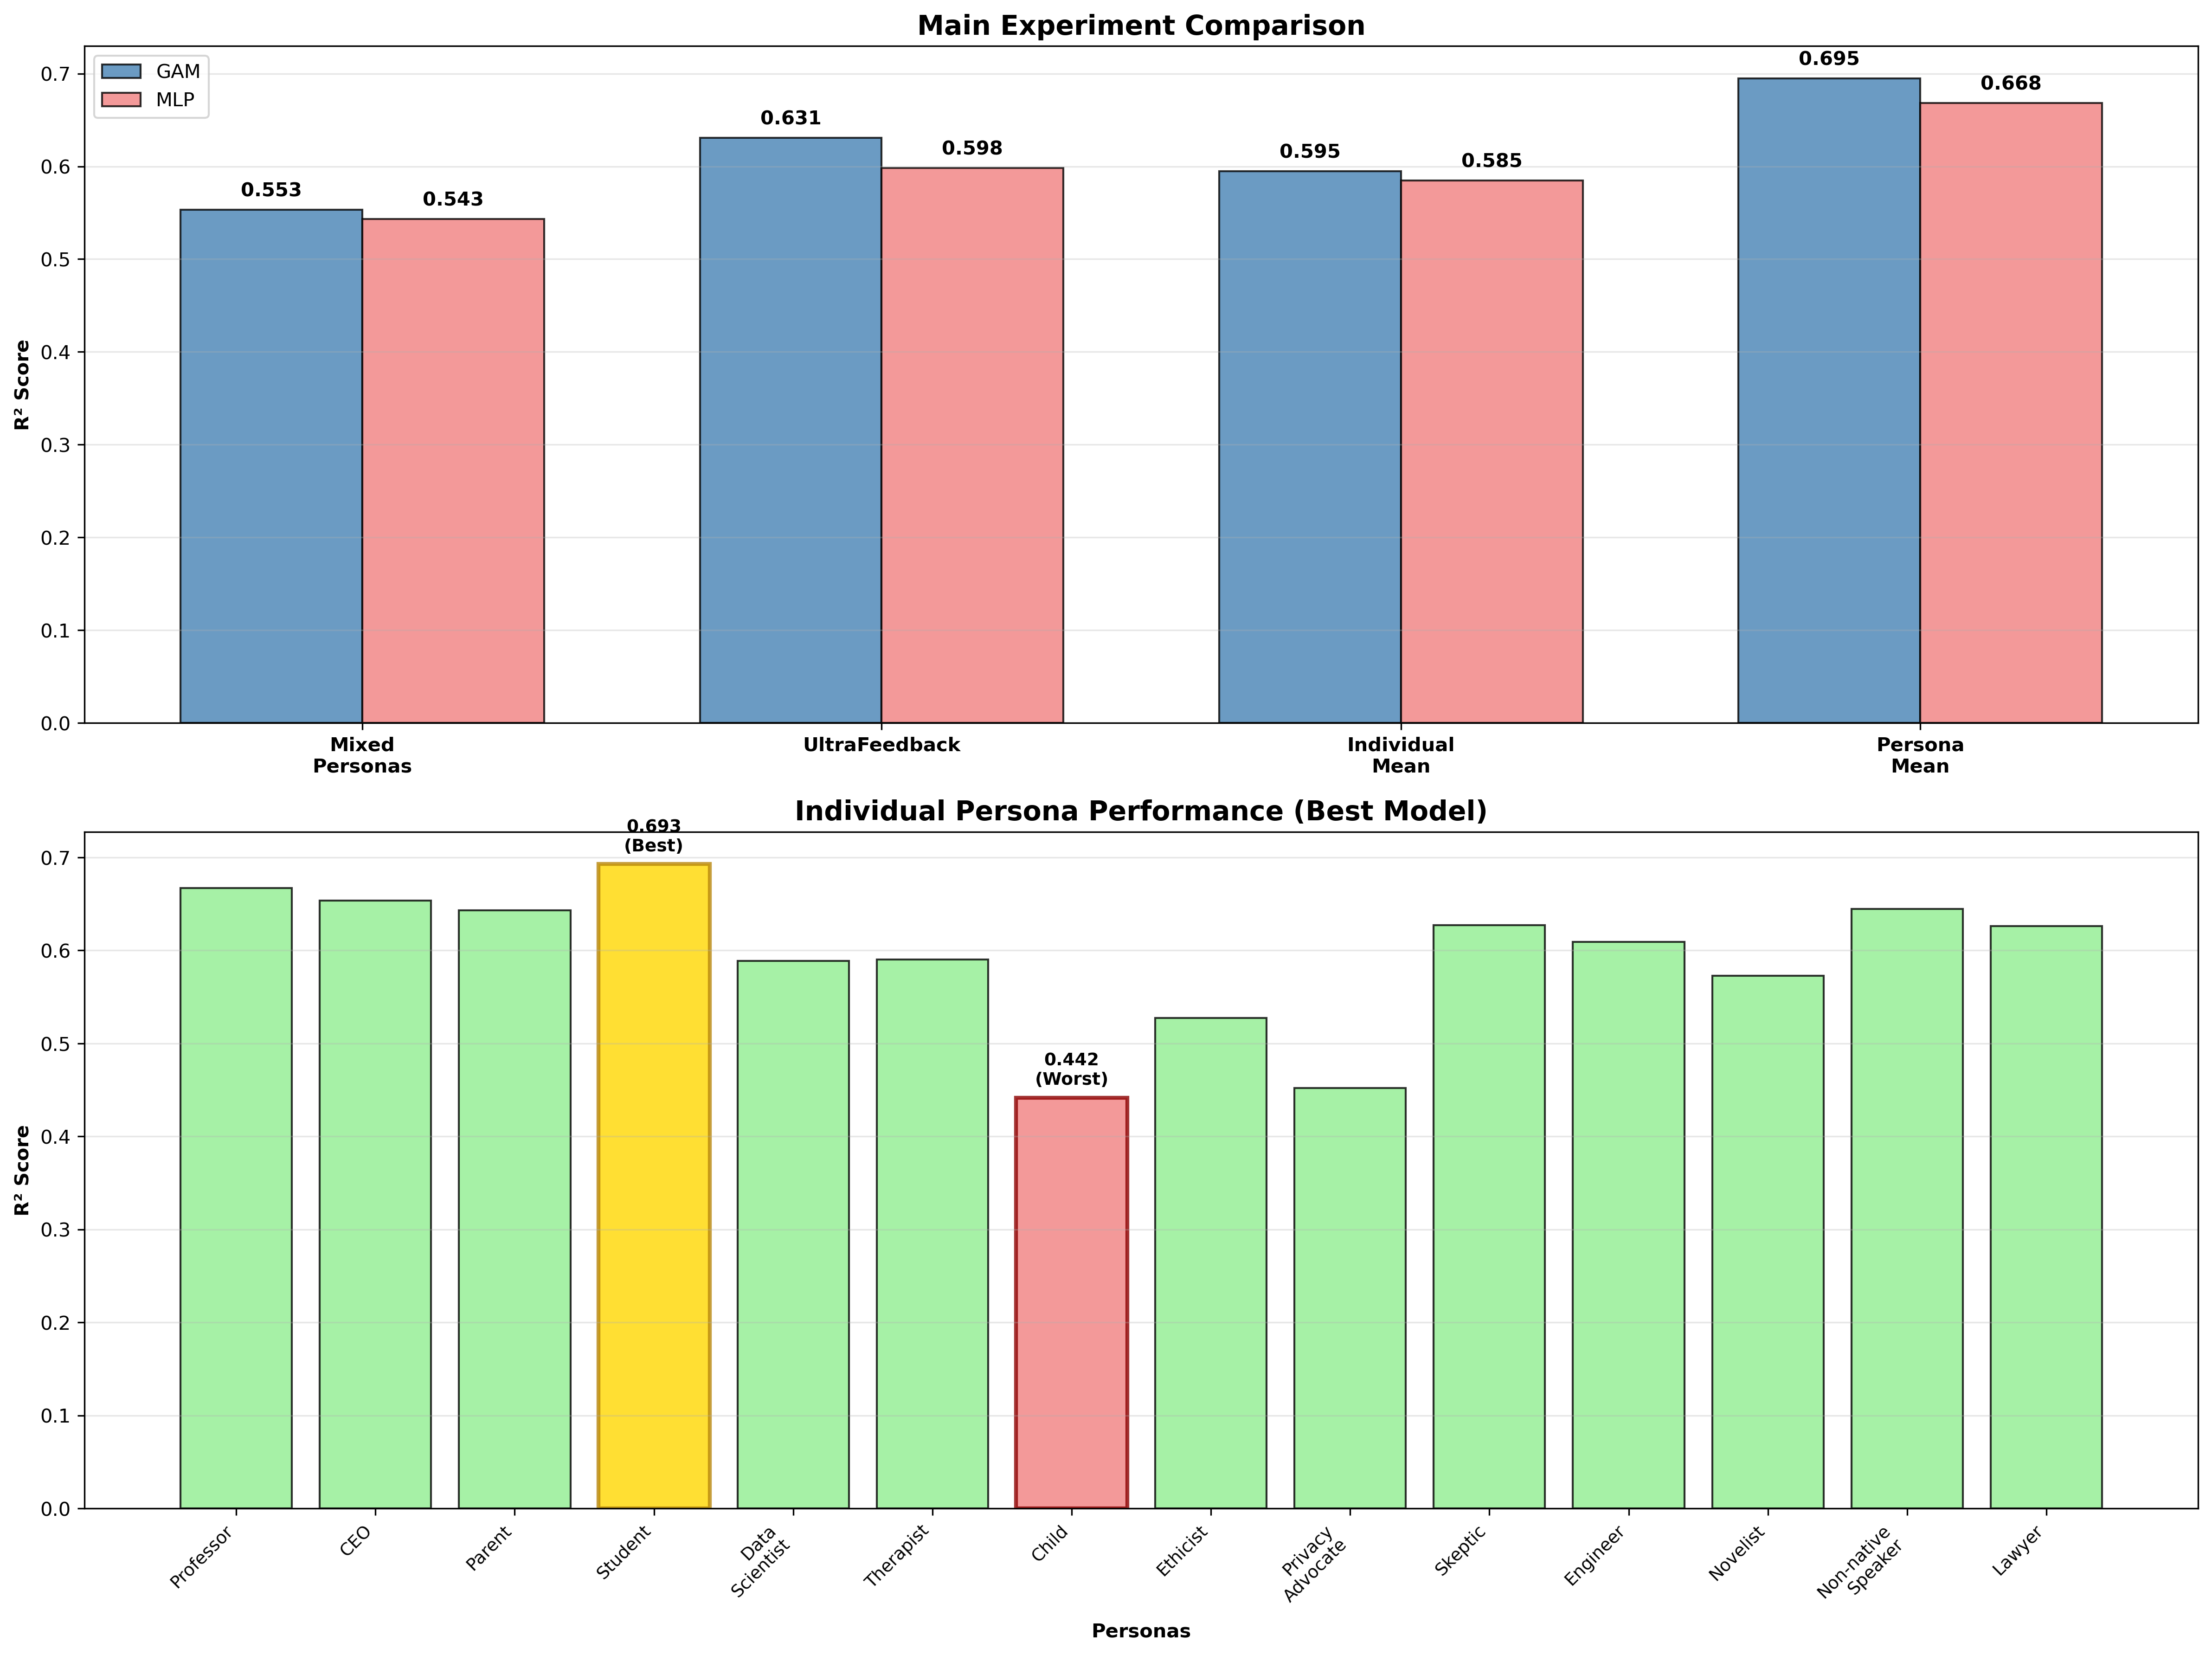
\includegraphics[width=\textwidth]{experiments/2b_aggregator_validation/experiment_results_full/plots/4_extended_comparison.png}
    \caption{Aggregator Performance Across Different Ground Truth Types: The top panel shows R² performance comparison across four ground truth types, with Persona Mean achieving the highest performance (GAM R² = 0.695). The bottom panel displays individual persona performance variation, with the Student persona achieving best results (R² = 0.693) and Child persona showing poorest alignment (R² = 0.442). This 25-percentage-point range reveals significant systematic differences in how well judge ensembles align with different human preference profiles.}
    \label{fig:variance_analysis_main}
\end{figure}

\begin{figure}[htbp]
    \centering
    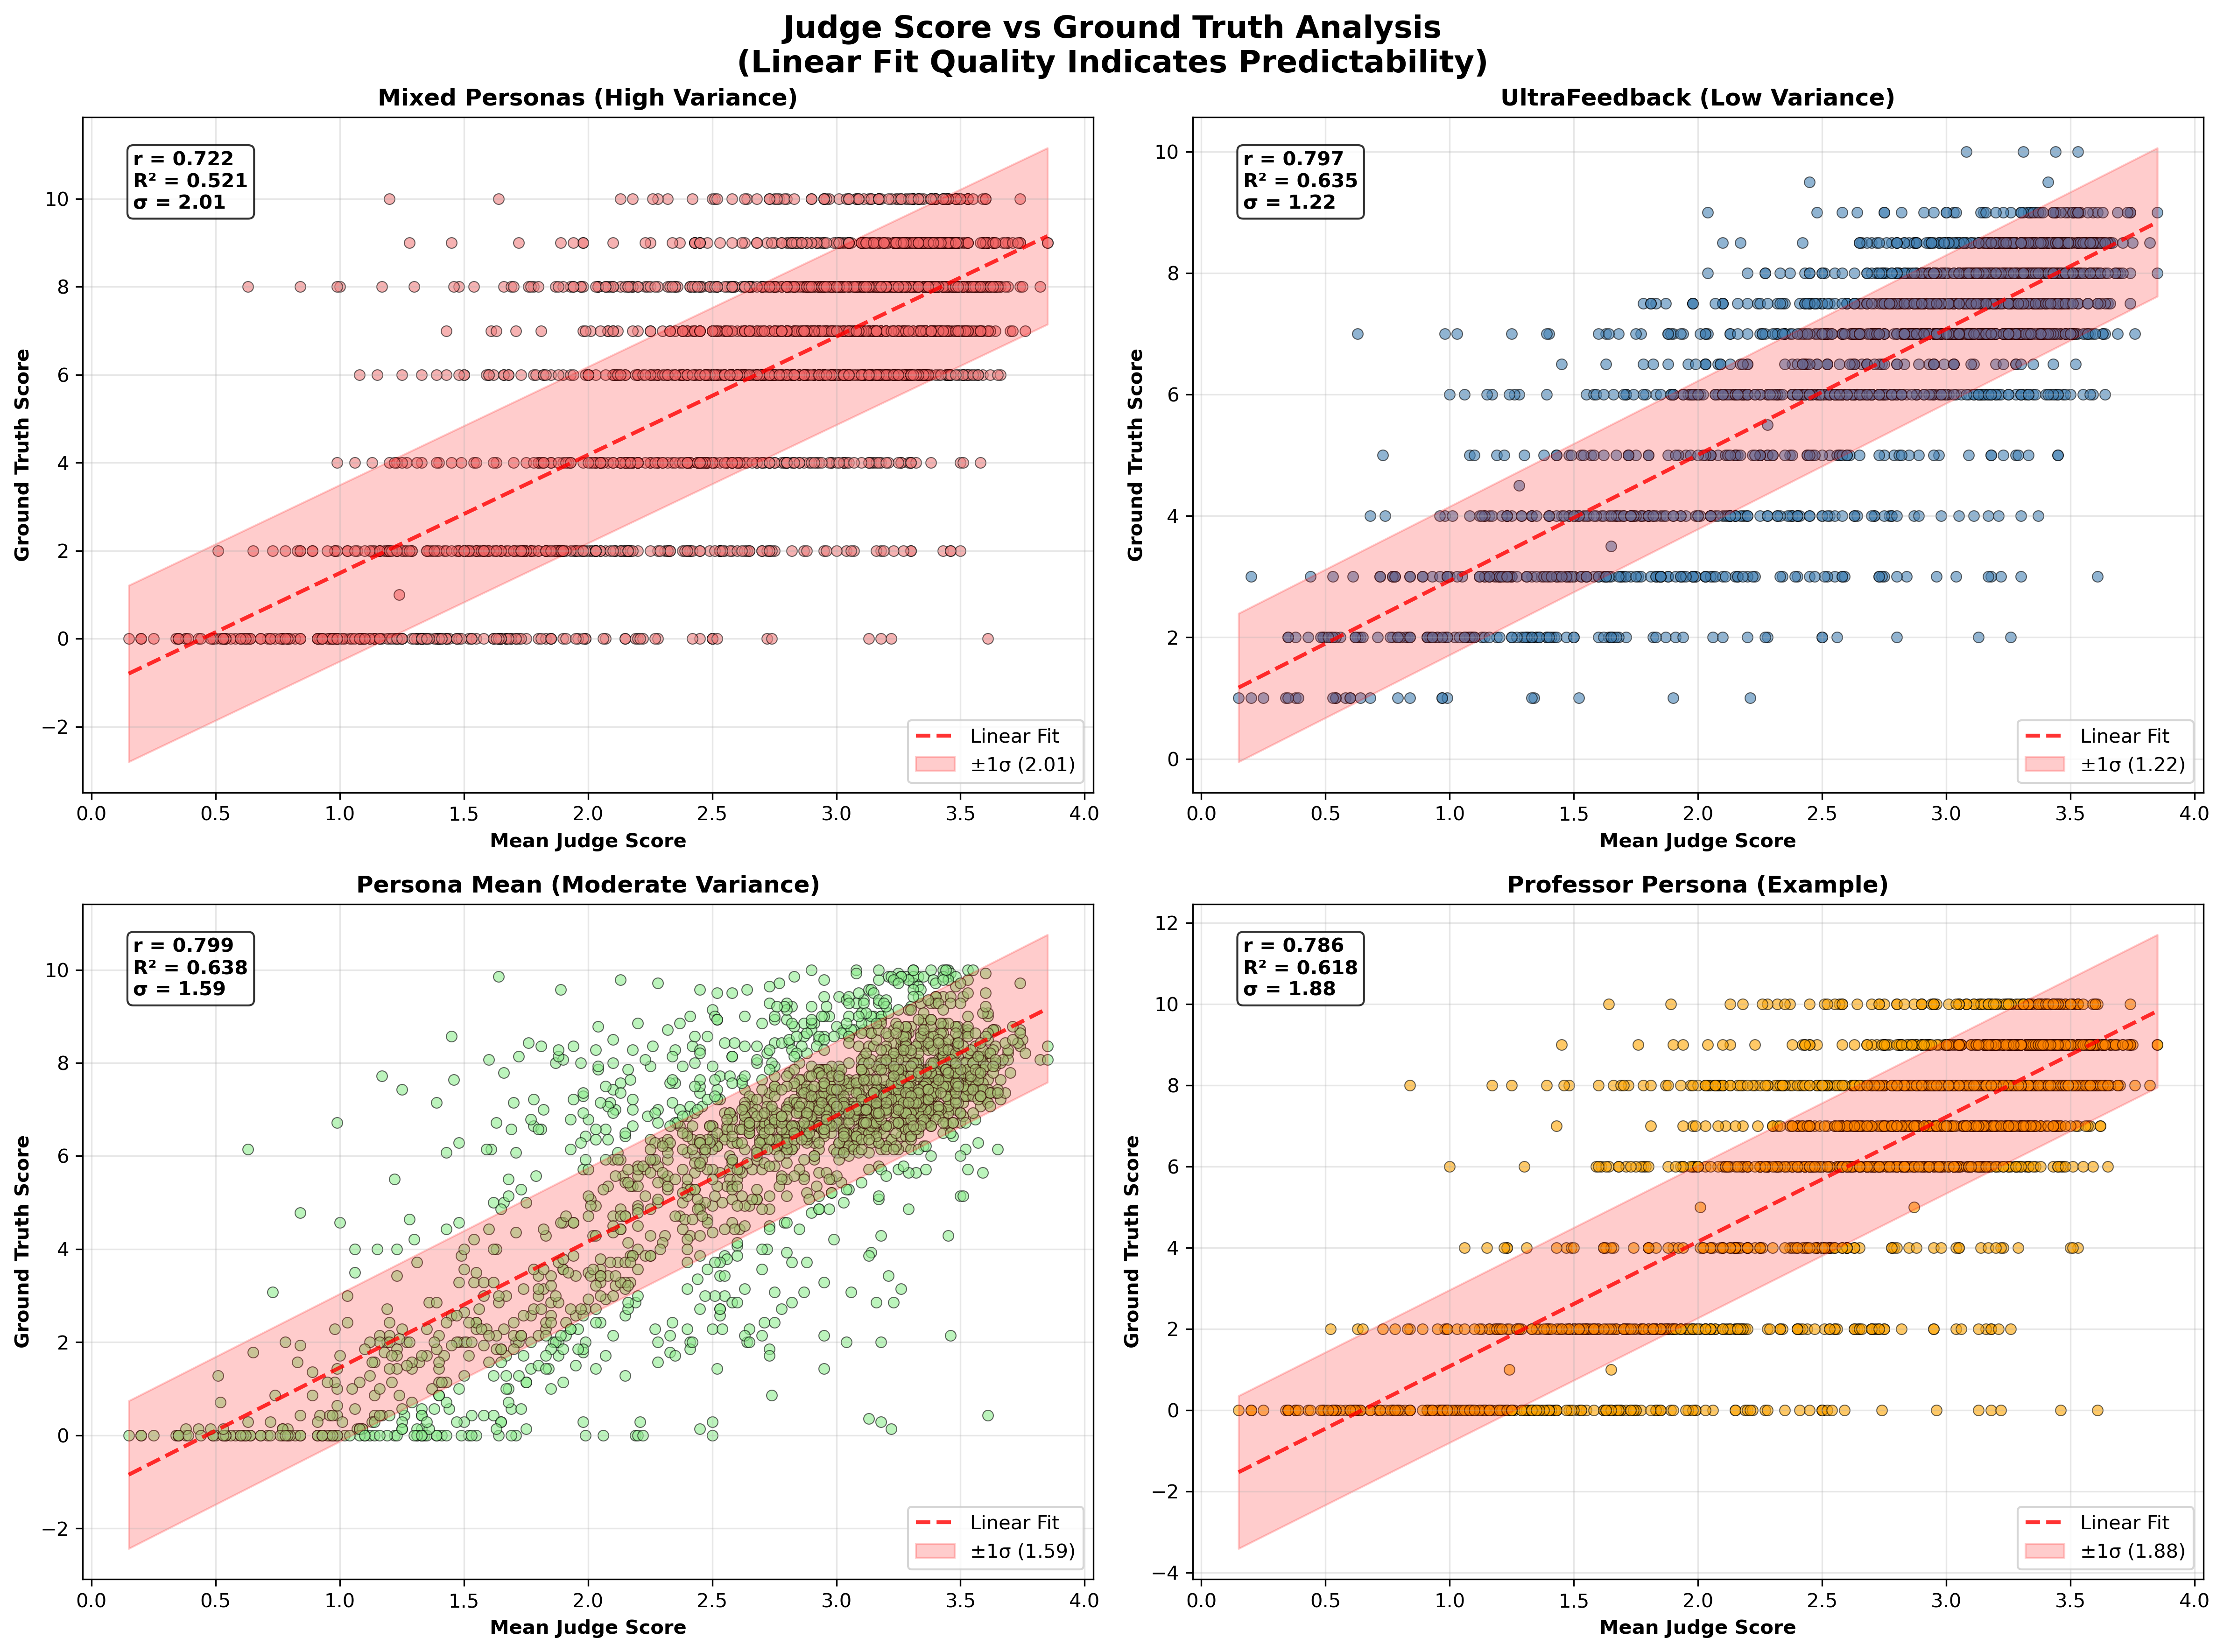
\includegraphics[width=\textwidth]{experiments/2b_aggregator_validation/experiment_results_full/plots/2_variance_scatter_analysis.png}
    \caption{Judge-Persona Alignment Analysis: Scatter plots revealing the relationship between mean judge scores and ground truth preferences across different ground truth conditions. The linear fit quality varies dramatically: UltraFeedback shows tight correlation (R = 0.89) due to single-model consistency, while our Mixed Personas approach exhibits higher variance (R = 0.62) reflecting diverse preference profiles. The correlation differences demonstrate that our diverse persona sampling methodology creates measurable alignment challenges, yet the modest performance gains from more consistent targets suggest the diversity provides valuable training signal that compensates for increased variance.}
    \label{fig:variance_scatter_analysis}
\end{figure}

The results reveal that our diverse persona sampling methodology is not the primary constraint on aggregator performance. Despite UltraFeedback representing consistent single-model preferences with 39\% lower variance than our Mixed Personas approach (4.98 vs 8.20), it achieved only moderate R² improvement (0.631 vs 0.553). Individual persona experiments, while internally consistent, performed even worse on average (R² = 0.595), demonstrating that preference consistency alone does not unlock superior aggregation.

Surprisingly, the Persona Mean condition achieved the highest performance (R² = 0.695), suggesting that our diverse sampling strategy actually captures valuable preference signal when properly aggregated. Rather than constraining performance, the diversity in our persona sampling appears to provide richer training signal that enables better generalization when combined optimally.

These findings validate our diverse persona sampling methodology while redirecting future research toward learning better persona-aware aggregation functions that can leverage the full spectrum of human preference diversity, rather than avoiding it through sampling constraints.

\subsection{Summary of Key Results}

Our experimental validation demonstrates:

\begin{enumerate}
    \item \textbf{Performance}: Learned aggregation achieves 15-16\% improvement over naive methods (MLP R² = 0.578, GAM R² = 0.575 vs. naive R² = 0.498)
    \item \textbf{Interpretability}: GAM provides transparency in judge contributions while maintaining competitive performance
    \item \textbf{Methodology Validation}: Our diverse persona sampling strategy is not constraining performance—it provides valuable training signal that enables better generalization when properly aggregated
    \item \textbf{Robustness}: System remains functional under up to 20\% contamination across multiple persona contamination strategies. [Pending Judge Robustness experiment results]
\end{enumerate}

These results validate our multi-judge interpretability framework as a practical approach for robust, transparent AI evaluation systems that outperform existing methods while providing actionable insights into evaluation quality and potential failure modes.
